%% bare_jrnl.tex
%% V1.4b
%% 2015/08/26
%% by Michael Shell
%% see http://www.michaelshell.org/
%% for current contact information.
%%
%% This is a skeleton file demonstrating the use of IEEEtran.cls
%% (requires IEEEtran.cls version 1.8b or later) with an IEEE
%% journal paper.
%%
%% Support sites:
%% http://www.michaelshell.org/tex/ieeetran/
%% http://www.ctan.org/pkg/ieeetran
%% and
%% http://www.ieee.org/

%%*************************************************************************
%% Legal Notice:
%% This code is offered as-is without any warranty either expressed or
%% implied; without even the implied warranty of MERCHANTABILITY or
%% FITNESS FOR A PARTICULAR PURPOSE! 
%% User assumes all risk.
%% In no event shall the IEEE or any contributor to this code be liable for
%% any damages or losses, including, but not limited to, incidental,
%% consequential, or any other damages, resulting from the use or misuse
%% of any information contained here.
%%
%% All comments are the opinions of their respective authors and are not
%% necessarily endorsed by the IEEE.
%%
%% This work is distributed under the LaTeX Project Public License (LPPL)
%% ( http://www.latex-project.org/ ) version 1.3, and may be freely used,
%% distributed and modified. A copy of the LPPL, version 1.3, is included
%% in the base LaTeX documentation of all distributions of LaTeX released
%% 2003/12/01 or later.
%% Retain all contribution notices and credits.
%% ** Modified files should be clearly indicated as such, including  **
%% ** renaming them and changing author support contact information. **
%%*************************************************************************


% *** Authors should verify (and, if needed, correct) their LaTeX system  ***
% *** with the testflow diagnostic prior to trusting their LaTeX platform ***
% *** with production work. The IEEE's font choices and paper sizes can   ***
% *** trigger bugs that do not appear when using other class files.       ***                          ***
% The testflow support page is at:
% http://www.michaelshell.org/tex/testflow/



\documentclass[journal]{IEEEtran}
%
% If IEEEtran.cls has not been installed into the LaTeX system files,
% manually specify the path to it like:
% \documentclass[journal]{../sty/IEEEtran}
\usepackage[flushleft]{threeparttable}
\usepackage{amsmath}
\usepackage{graphicx}
\usepackage{tikz}
\usepackage{pgfplots,pgfplotstable}
\usepackage{pdfpages}
%\usepackage{tikz}
\usepackage{algorithm}
\usepackage[colorinlistoftodos]{todonotes}
\usepackage[colorlinks=true, allcolors=blue, breaklinks=true]{hyperref}
\usepackage[noend]{algorithmic}
\usepackage{mathtools}
\usepackage{multirow}
%\usepackage{mathabx}
%\usetikzlibrary{intersections}

\newcommand{\COMB}{{\sc comb}}
\newcommand{\DCS}{{\sc dcs}}
\newcommand{\EA}{{\sc ea}}
\newcommand{\EAS}{{\sc ea}s}
\newcommand{\GDEIII}{{\sc gde3}}
\newcommand{\HGSADC}{{\sc hgsadc}}
\newcommand{\MOEA}{{\sc moea}}
\newcommand{\MOEAD}{{\sc moea/d}}
\newcommand{\MOEAS}{{\sc moea}s}
\newcommand{\MOP}{{\sc mop}}
\newcommand{\MOPS}{{\sc mop}s}
\newcommand{\NSGAII}{{\sc nsga-ii}}
\newcommand{\IBEA}{{\sc ibea}}
\newcommand{\VSDMOEA}{{\sc vsd-moea}}
\newcommand{\RMOEA}{{\sc r2-emoa}}
\newcommand{\WFG}{{\sc wfg}}
\newcommand{\AASF}{{\sc aasf}}
\newcommand{\HV}{{\sc hv}}


%%%%%%%%%%%%%data

%\pgfplotsset{compat=1.3}


% Some very useful LaTeX packages include:
% (uncomment the ones you want to load)


% *** MISC UTILITY PACKAGES ***
%
%\usepackage{ifpdf}
% Heiko Oberdiek's ifpdf.sty is very useful if you need conditional
% compilation based on whether the output is pdf or dvi.
% usage:
% \ifpdf
%   % pdf code
% \else
%   % dvi code
% \fi
% The latest version of ifpdf.sty can be obtained from:
% http://www.ctan.org/pkg/ifpdf
% Also, note that IEEEtran.cls V1.7 and later provides a builtin
% \ifCLASSINFOpdf conditional that works the same way.
% When switching from latex to pdflatex and vice-versa, the compiler may
% have to be run twice to clear warning/error messages.






% *** CITATION PACKAGES ***
%
%\usepackage{cite}
% cite.sty was written by Donald Arseneau
% V1.6 and later of IEEEtran pre-defines the format of the cite.sty package
% \cite{} output to follow that of the IEEE. Loading the cite package will
% result in citation numbers being automatically sorted and properly
% "compressed/ranged". e.g., [1], [9], [2], [7], [5], [6] without using
% cite.sty will become [1], [2], [5]--[7], [9] using cite.sty. cite.sty's
% \cite will automatically add leading space, if needed. Use cite.sty's
% noadjust option (cite.sty V3.8 and later) if you want to turn this off
% such as if a citation ever needs to be enclosed in parenthesis.
% cite.sty is already installed on most LaTeX systems. Be sure and use
% version 5.0 (2009-03-20) and later if using hyperref.sty.
% The latest version can be obtained at:
% http://www.ctan.org/pkg/cite
% The documentation is contained in the cite.sty file itself.






% *** GRAPHICS RELATED PACKAGES ***
%
\ifCLASSINFOpdf
  % \usepackage[pdftex]{graphicx}
  % declare the path(s) where your graphic files are
  % \graphicspath{{../pdf/}{../jpeg/}}
  % and their extensions so you won't have to specify these with
  % every instance of \includegraphics
  % \DeclareGraphicsExtensions{.pdf,.jpeg,.png}
\else
  % or other class option (dvipsone, dvipdf, if not using dvips). graphicx
  % will default to the driver specified in the system graphics.cfg if no
  % driver is specified.
  % \usepackage[dvips]{graphicx}
  % declare the path(s) where your graphic files are
  % \graphicspath{{../eps/}}
  % and their extensions so you won't have to specify these with
  % every instance of \includegraphics
  % \DeclareGraphicsExtensions{.eps}
\fi
% graphicx was written by David Carlisle and Sebastian Rahtz. It is
% required if you want graphics, photos, etc. graphicx.sty is already
% installed on most LaTeX systems. The latest version and documentation
% can be obtained at: 
% http://www.ctan.org/pkg/graphicx
% Another good source of documentation is "Using Imported Graphics in
% LaTeX2e" by Keith Reckdahl which can be found at:
% http://www.ctan.org/pkg/epslatex
%
% latex, and pdflatex in dvi mode, support graphics in encapsulated
% postscript (.eps) format. pdflatex in pdf mode supports graphics
% in .pdf, .jpeg, .png and .mps (metapost) formats. Users should ensure
% that all non-photo figures use a vector format (.eps, .pdf, .mps) and
% not a bitmapped formats (.jpeg, .png). The IEEE frowns on bitmapped formats
% which can result in "jaggedy"/blurry rendering of lines and letters as
% well as large increases in file sizes.
%
% You can find documentation about the pdfTeX application at:
% http://www.tug.org/applications/pdftex





% *** MATH PACKAGES ***
%
%\usepackage{amsmath}
% A popular package from the American Mathematical Society that provides
% many useful and powerful commands for dealing with mathematics.
%
% Note that the amsmath package sets \interdisplaylinepenalty to 10000
% thus preventing page breaks from occurring within multiline equations. Use:
%\interdisplaylinepenalty=2500
% after loading amsmath to restore such page breaks as IEEEtran.cls normally
% does. amsmath.sty is already installed on most LaTeX systems. The latest
% version and documentation can be obtained at:
% http://www.ctan.org/pkg/amsmath





% *** SPECIALIZED LIST PACKAGES ***
%
%\usepackage{algorithmic}
% algorithmic.sty was written by Peter Williams and Rogerio Brito.
% This package provides an algorithmic environment fo describing algorithms.
% You can use the algorithmic environment in-text or within a figure
% environment to provide for a floating algorithm. Do NOT use the algorithm
% floating environment provided by algorithm.sty (by the same authors) or
% algorithm2e.sty (by Christophe Fiorio) as the IEEE does not use dedicated
% algorithm float types and packages that provide these will not provide
% correct IEEE style captions. The latest version and documentation of
% algorithmic.sty can be obtained at:
% http://www.ctan.org/pkg/algorithms
% Also of interest may be the (relatively newer and more customizable)
% algorithmicx.sty package by Szasz Janos:
% http://www.ctan.org/pkg/algorithmicx




% *** ALIGNMENT PACKAGES ***
%
%\usepackage{array}
% Frank Mittelbach's and David Carlisle's array.sty patches and improves
% the standard LaTeX2e array and tabular environments to provide better
% appearance and additional user controls. As the default LaTeX2e table
% generation code is lacking to the point of almost being broken with
% respect to the quality of the end results, all users are strongly
% advised to use an enhanced (at the very least that provided by array.sty)
% set of table tools. array.sty is already installed on most systems. The
% latest version and documentation can be obtained at:
% http://www.ctan.org/pkg/array


% IEEEtran contains the IEEEeqnarray family of commands that can be used to
% generate multiline equations as well as matrices, tables, etc., of high
% quality.




% *** SUBFIGURE PACKAGES ***
%\ifCLASSOPTIONcompsoc
%  \usepackage[caption=false,font=normalsize,labelfont=sf,textfont=sf]{subfig}
%\else
%  \usepackage[caption=false,font=footnotesize]{subfig}
%\fi
% subfig.sty, written by Steven Douglas Cochran, is the modern replacement
% for subfigure.sty, the latter of which is no longer maintained and is
% incompatible with some LaTeX packages including fixltx2e. However,
% subfig.sty requires and automatically loads Axel Sommerfeldt's caption.sty
% which will override IEEEtran.cls' handling of captions and this will result
% in non-IEEE style figure/table captions. To prevent this problem, be sure
% and invoke subfig.sty's "caption=false" package option (available since
% subfig.sty version 1.3, 2005/06/28) as this is will preserve IEEEtran.cls
% handling of captions.
% Note that the Computer Society format requires a larger sans serif font
% than the serif footnote size font used in traditional IEEE formatting
% and thus the need to invoke different subfig.sty package options depending
% on whether compsoc mode has been enabled.
%
% The latest version and documentation of subfig.sty can be obtained at:
% http://www.ctan.org/pkg/subfig




% *** FLOAT PACKAGES ***
%
%\usepackage{fixltx2e}
% fixltx2e, the successor to the earlier fix2col.sty, was written by
% Frank Mittelbach and David Carlisle. This package corrects a few problems
% in the LaTeX2e kernel, the most notable of which is that in current
% LaTeX2e releases, the ordering of single and double column floats is not
% guaranteed to be preserved. Thus, an unpatched LaTeX2e can allow a
% single column figure to be placed prior to an earlier double column
% figure.
% Be aware that LaTeX2e kernels dated 2015 and later have fixltx2e.sty's
% corrections already built into the system in which case a warning will
% be issued if an attempt is made to load fixltx2e.sty as it is no longer
% needed.
% The latest version and documentation can be found at:
% http://www.ctan.org/pkg/fixltx2e


%\usepackage{stfloats}
% stfloats.sty was written by Sigitas Tolusis. This package gives LaTeX2e
% the ability to do double column floats at the bottom of the page as well
% as the top. (e.g., "\begin{figure*}[!b]" is not normally possible in
% LaTeX2e). It also provides a command:
%\fnbelowfloat
% to enable the placement of footnotes below bottom floats (the standard
% LaTeX2e kernel puts them above bottom floats). This is an invasive package
% which rewrites many portions of the LaTeX2e float routines. It may not work
% with other packages that modify the LaTeX2e float routines. The latest
% version and documentation can be obtained at:
% http://www.ctan.org/pkg/stfloats
% Do not use the stfloats baselinefloat ability as the IEEE does not allow
% \baselineskip to stretch. Authors submitting work to the IEEE should note
% that the IEEE rarely uses double column equations and that authors should try
% to avoid such use. Do not be tempted to use the cuted.sty or midfloat.sty
% packages (also by Sigitas Tolusis) as the IEEE does not format its papers in
% such ways.
% Do not attempt to use stfloats with fixltx2e as they are incompatible.
% Instead, use Morten Hogholm'a dblfloatfix which combines the features
% of both fixltx2e and stfloats:
%
% \usepackage{dblfloatfix}
% The latest version can be found at:
% http://www.ctan.org/pkg/dblfloatfix




%\ifCLASSOPTIONcaptionsoff
%  \usepackage[nomarkers]{endfloat}
% \let\MYoriglatexcaption\caption
% \renewcommand{\caption}[2][\relax]{\MYoriglatexcaption[#2]{#2}}
%\fi
% endfloat.sty was written by James Darrell McCauley, Jeff Goldberg and 
% Axel Sommerfeldt. This package may be useful when used in conjunction with 
% IEEEtran.cls'  captionsoff option. Some IEEE journals/societies require that
% submissions have lists of figures/tables at the end of the paper and that
% figures/tables without any captions are placed on a page by themselves at
% the end of the document. If needed, the draftcls IEEEtran class option or
% \CLASSINPUTbaselinestretch interface can be used to increase the line
% spacing as well. Be sure and use the nomarkers option of endfloat to
% prevent endfloat from "marking" where the figures would have been placed
% in the text. The two hack lines of code above are a slight modification of
% that suggested by in the endfloat docs (section 8.4.1) to ensure that
% the full captions always appear in the list of figures/tables - even if
% the user used the short optional argument of \caption[]{}.
% IEEE papers do not typically make use of \caption[]'s optional argument,
% so this should not be an issue. A similar trick can be used to disable
% captions of packages such as subfig.sty that lack options to turn off
% the subcaptions:
% For subfig.sty:
% \let\MYorigsubfloat\subfloat
% \renewcommand{\subfloat}[2][\relax]{\MYorigsubfloat[]{#2}}
% However, the above trick will not work if both optional arguments of
% the \subfloat command are used. Furthermore, there needs to be a
% description of each subfigure *somewhere* and endfloat does not add
% subfigure captions to its list of figures. Thus, the best approach is to
% avoid the use of subfigure captions (many IEEE journals avoid them anyway)
% and instead reference/explain all the subfigures within the main caption.
% The latest version of endfloat.sty and its documentation can obtained at:
% http://www.ctan.org/pkg/endfloat
%
% The IEEEtran \ifCLASSOPTIONcaptionsoff conditional can also be used
% later in the document, say, to conditionally put the References on a 
% page by themselves.




% *** PDF, URL AND HYPERLINK PACKAGES ***
%
%\usepackage{url}
% url.sty was written by Donald Arseneau. It provides better support for
% handling and breaking URLs. url.sty is already installed on most LaTeX
% systems. The latest version and documentation can be obtained at:
% http://www.ctan.org/pkg/url
% Basically, \url{my_url_here}.




% *** Do not adjust lengths that control margins, column widths, etc. ***
% *** Do not use packages that alter fonts (such as pslatex).         ***
% There should be no need to do such things with IEEEtran.cls V1.6 and later.
% (Unless specifically asked to do so by the journal or conference you plan
% to submit to, of course. )


% correct bad hyphenation here
\hyphenation{op-tical net-works semi-conduc-tor}


\begin{document}
%
% paper title
% Titles are generally capitalized except for words such as a, an, and, as,
% at, but, by, for, in, nor, of, on, or, the, to and up, which are usually
% not capitalized unless they are the first or last word of the title.
% Linebreaks \\ can be used within to get better formatting as desired.
% Do not put math or special symbols in the title.
\title{Supplementary Document for ``VSD-MOEA: A Dominance-Based Multi-Objective Evolutionary Algorithm with Explicit Variable Space Diversity Management''}
%
%
% author names and IEEE memberships
% note positions of commas and nonbreaking spaces ( ~ ) LaTeX will not break
% a structure at a ~ so this keeps an author's name from being broken across
% two lines.
% use \thanks{} to gain access to the first footnote area
% a separate \thanks must be used for each paragraph as LaTeX2e's \thanks
% was not built to handle multiple paragraphs
%

\author{Joel~Chac\'on~Castillo,
        Carlos~Segura,~\IEEEmembership{Member,~IEEE,}
        %,~\IEEEmembership{Fellow,~OSA,}
        and~Carlos A. Coello Coello,~\IEEEmembership{Fellow,~IEEE,}
        %and~Arturo~Hern\'andez-Aguirre%~\IEEEmembership{Life~Fellow,~IEEE}% <-this % stops a space
\thanks{J. Chac\'on, and C. Segura are with the Center for Research in Mathematics (CIMAT), Computer Science Department,
Callej\'on Jalisco s/n, Mineral de Valenciana, Guanajuato, Guanajuato 36240, Mexico (e-mail: joel.chacon@cimat.mx; carlos.segura@cimat.mx)}%
\thanks{C. A. Coello Coello is with the Evolutionary Computation
Group, Computer Science Department, CINVESTAV-IPN, Mexico City 07300, 
Mexico (e-mail: ccoello@cs.cinvestav.mx).}% <-this % stops a space
\thanks{Digital Object Identifier xxx}
\thanks{Manuscript received XX, XX 2019; revised XX XX, XX.}%
}

% note the % following the last \IEEEmembership and also \thanks - 
% these prevent an unwanted space from occurring between the last author name
% and the end of the author line. i.e., if you had this:
% 
% \author{....lastname \thanks{...} \thanks{...} }
%                     ^------------^------------^----Do not want these spaces!
%
% a space would be appended to the last name and could cause every name on that
% line to be shifted left slightly. This is one of those "LaTeX things". For
% instance, "\textbf{A} \textbf{B}" will typeset as "A B" not "AB". To get
% "AB" then you have to do: "\textbf{A}\textbf{B}"
% \thanks is no different in this regard, so shield the last } of each \thanks
% that ends a line with a % and do not let a space in before the next \thanks.
% Spaces after \IEEEmembership other than the last one are OK (and needed) as
% you are supposed to have spaces between the names. For what it is worth,
% this is a minor point as most people would not even notice if the said evil
% space somehow managed to creep in.



% The paper headers


\markboth{IEEE Transactions on Cybernetics,~Vol.~XX, No.~X, Month~Year}{Chacón \MakeLowercase{\textit{et al.}}: Supplementary Document for ''VSD-MOEA: A Dominance-Based Multi-Objective Evolutionary Algorithm with Explicit Variable Space Diversity Management``}

% The only time the second header will appear is for the odd numbered pages
% after the title page when using the twoside option.
% 
% *** Note that you probably will NOT want to include the author's ***
% *** name in the headers of peer review papers.                   ***
% You can use \ifCLASSOPTIONpeerreview for conditional compilation here if
% you desire.




% If you want to put a publisher's ID mark on the page you can do it like
% this:
%\IEEEpubid{0000--0000/00\$00.00~\copyright~2015 IEEE}
% Remember, if you use this you must call \IEEEpubidadjcol in the second
% column for its text to clear the IEEEpubid mark.



% use for special paper notices
%\IEEEspecialpapernotice{(Invited Paper)}




% make the title area
\maketitle

% As a general rule, do not put math, special symbols or citations
% in the abstract or keywords.
%\begin{abstract}
%Most state-of-the-art Multi-Objective Evolutionary Algorithms (\MOEAS{}) promote the preservation of diversity 
of objective function space but neglects the diversity of decision variable space.
%
The aim of this paper is to show that controlling explicitly the amount of diversity maintained in the decision variable space 
is useful to increase the quality of \MOEAS{} when taking into account metrics of the objective space.
%
Our novel Variable Space Diversity based MOEA (\VSDMOEA{})
explicitly considers the diversity of both decision variable and objective function space.
%
This information is used with the aim of properly adapting the balance between exploration
and intensification during the optimization process.
%
Particularly, at the initial stages, decisions made by the approach are more biased by the information on the diversity of 
the variable space, whereas it gradually grants more importance to the diversity of objective function space as the 
evolution progresses.
%
The latter is achieved through a novel density estimator.
%
The new method is compared with state-of-art \MOEAS{} using several benchmarks with two and three objectives.
%
This novel proposal yields much better results than state-of-the-art schemes when considering metrics applied on 
objective function space, exhibiting a more stable and robust behavior.

%\end{abstract}

% Note that keywords are not normally used for peerreview papers.
%\begin{IEEEkeywords}
%IEEE, IEEEtran, journal, \LaTeX, paper, template.
%\end{IEEEkeywords}






% For peer review papers, you can put extra information on the cover
% page as needed:
% \ifCLASSOPTIONpeerreview
% \begin{center} \bfseries EDICS Category: 3-BBND \end{center}
% \fi
%
% For peerreview papers, this IEEEtran command inserts a page break and
% creates the second title. It will be ignored for other modes.
\IEEEpeerreviewmaketitle



%\section{Introduction}
%\IEEEPARstart{M}{ulti-objective} Optimization Problems (\MOPS{}) %have a number of objective functions which are to be minimized or maximized.
%
%Thus, differently to single-objective optimization, \MOPS{} 
involve the simultaneous optimization of several objective functions that are usually in conflict~\cite{Joel:Kalyanmoy}. 
%
A continuous box-constrained minimization \MOP{}, which is the kind of problem addressed in this paper, can be defined as follows:
\begin{equation}
   \begin{split}
    minimize \quad & \vec{F} = [f_1(\vec{\mathbf{x}}), f_2(\vec{\mathbf{x}}), ..., f_M(\vec{\mathbf{x}})] \\
   subject \quad to \quad &  x_i^{(L)} \leq x_i \leq x_i^{(U)}, \quad i=1,2,..., n. \\
   %& \vec{\mathbf{x}} \in \Omega
   \end{split}
\end{equation}
where $n$ corresponds to the dimension of the variable space, $\vec{\mathbf{x}}$ is a vector of $n$ 
variables $\vec{\mathbf{x}}=(x_1, ..., x_n) \in R^n$, which are constrained by $x_i^{(L)}$ 
and $x_i^{(U)}$, i.e. the lower bound and upper bound, and $M$ is the number of objective functions
to optimize.
%
The feasible space bounded by $x_i^{(L)}$ and $x_i^{(U)}$ is denoted by $\Omega$,
each solution is mapped to the objective space with the function $F : \Omega \rightarrow R^M$, 
which consist of $M$ real-valued objective functions and $R^M$ is called the \textit{objective space}. 

Given two solutions $\vec{\mathbf{x}}$, $\vec{\mathbf{y}}$ $\in \Omega$, $\vec{\mathbf{x}}$ dominates $\vec{\mathbf{y}}$, 
mathematically denoted by $\vec{\mathbf{x}} \prec \vec{\mathbf{y}}$, iff $\forall m \in {1,2,...,M} : 
f_m(\vec{\mathbf{x}}) \leq f_m(\vec{\mathbf{y}})$ and $\exists  m \in {1,2,...,M} : f_m(\vec{\mathbf{x}}) < f_m(\vec{\mathbf{y}})$.
%
The best solutions of a \MOP{} are those that are not dominated by any other feasible vector.
%
These solutions are known as the Pareto optimal solutions.
%
The Pareto set is the set of all Pareto optimal solutions, and the Pareto front are the images of the Pareto set. 
%
The goal of most multi-objective optimizers is to obtain a proper approximation of the Pareto front, i.e., 
a set of well distributed solutions that are close to the Pareto front.

One of the most popular meta-heuristics used to deal with \MOPS{} is the Evolutionary Algorithm (\EA{}).
%
In single-objective \EAS{}, it has been shown that taking into account the diversity of the variable space
to properly balance between exploration and exploitation is highly important to attain high quality 
solutions~\cite{Joel:BALANCE_DIVERSITY}.
%
Diversity can be taken into account in the design of several components such as in the variation 
stage~\cite{Joel:FUZZY_ADAPTIVE_GA,Joel:CROSSOVER_DIVERSITY}, replacement phase~\cite{Joel:MULTI_DYNAMIC} 
and/or population model~\cite{Joel:SAWTOOTH}.
%In the uniprocess-driven proposals only one component is affected, whereas in the multiprocess-driven ones, several components are redesigned~\cite{Joel:Crepinsek}. 
%
%One of the key issues that affects the performance of population-based metaheuristics is the premature convergence, which appears
%when most of the population members are placed in a small region of the search space and the components selected do not allow escaping from this region.
%
The explicit consideration of diversity leads to improvements in terms of premature convergence avoidance, 
meaning that taking into account the diversity in the design of \EAS{} is specially important when dealing 
with long-term executions.
%
Recently, some diversity management algorithms that combine the information of diversity, stopping criterion and elapsed 
generations have been devised.
%
They have allowed to provide a gradual loss of diversity that depends on the time or evaluations granted to the 
execution~\cite{Joel:MULTI_DYNAMIC}.
%
Particularly the aim of such a methodology is to promote exploration in the initial generations and gradually alter the 
behavior towards intensification.
%
These schemes have provided really promising results.
%
For instance, new best-known solutions for some well-known variants of the frequency assignment problem~\cite{Segura:17},
and for a two-dimensional packing problem~\cite{Joel:MULTI_DYNAMIC} have been attained using the same principles.
%
Additionally, this principle guided the design of the winning strategy of the Second Wind Farm Layout Optimization 
Competition\footnote{https://www.irit.fr/wind-competition/}, which was held in the Genetic and Evolutionary 
Computation Conference.
%
Thus, the benefits of such kind of design patterns have been shown in several different single-objective optimization problems.

One of the goals in the design of Multi-objective Evolutionary Algorithms (\MOEAS{}) is to obtain a well-spread 
set of solutions in the objective space.
%
As a result, most state-of-the-art \MOEAS{} consider the diversity of the objective space explicity.
%
However, this is not the case for the diversity of the variable space.
%
The maintenance of some degree of diversity of the objective space implies that complete convergence 
does not appear in the variable space~\cite{Joel:GDE3_CEC09}.
%
In some way, the variable space inherits some degree of diversity due to the way in which the objective space is 
taken into account. 
%
However, this is just an indirect way of preserving the diversity of the variable space, so 
in some cases the level of diversity might not be large enough to ensure a proper degree of exploration.
%
For instance, it has been shown that with some of the \WFG{} benchmarks, in most the state-of-the-art \MOEAS{} 
the \textit{distance parameters} quickly converge, meaning that the approach focuses just on optimizing the 
\textit{position parameters} for a long period of the optimization process~\cite{Joel:GDE3_CEC09}.
%
Thus, while some degree of diversity is maintained, a similar situation to premature convergence is presented
meaning that genetic operators might not be able to generate better trade-offs. 

Attending to the differences between state-of-the-art single-objective \EAS{} and \MOEAS{}, 
this paper proposes a novel \MOEA{}, the Variable Space Diversity based \MOEA{} (\VSDMOEA{}), 
that is based on controlling the amount of diversity of the variable space in an explicit way.
%
Similarly to the successful methodology applied in single-objective optimization, the stopping criterion and the 
amount of evaluations performed are used to vary the amount of desired diversity of the variable space.
%
The main difference with respect to the single-objective case is that the diversity of the objective space is simultaneously considered, 
which is performed with a novel objective space density estimator.
%
Particularly, the approach grants more importance to the diversity of the variable space in the initial stages, whereas 
as the generations evolve, it gradually grants more importance to the diversity of the objective space.
%
In fact, at the last period of the execution, the diversity of the variable space is neglected, so in the last phases the proposal 
is quite similar to current state-of-the-art approaches.
%
To our knowledge, this is the first \MOEA{} whose design follows this adaptive principle.
%
Since there exist currently a quite large amount of different \MOEAS{}~\cite{Joel:MOEA_APPLICATIONS_BOOK_KCTAN}, 
three popular schemes have been selected to validate our proposal.
%
%Most current taxonomies classify \MOEAS{} into three categories: non-domination based, based on decomposition and based on metrics.
%
%An approach of each of these categories was selected.
%
%Particularly, they are the Non-Dominated Sorting Genetic Algorithm II (NSGA-II)~\cite{Joel:NSGAII}, the \MOEA{} based on decomposition (\MOEAD{})~\cite{Joel:MOEAD}, 
%and the Many-Objective Genetic Algorithm Based on the R2 Indicator (MOMBI-II)~\cite{Joel:MOMBI-II}.
%
%Additionally, the Generalized Differential Evolution (GDE3)~\cite{Joel:GDE3}, which have a particularly different variation stage that has reported much benefits in several cases,
%is also included.
%
This validation has been performed with several well-known benchmarks and proper quality metrics.
%
The important benefits of properly taking into account the diversity of the variable space is
clearly shown in this paper.
%
Particularly, the advantages are clearer in the most complex problems.
%
Note that this is consistent with the single-objective case, where the most important benefits have been obtained
in complex multi-modal cases~\cite{Segura:17}.

The rest of this paper is organized as follows. 
%
Section~\ref{Sec:LiteratureReview} provides a review of related papers.
%
Some key components related to diversity and to the \VSDMOEA{} design are discussed.
%
The \VSDMOEA{} proposal is detailed in section~\ref{Sec:Proposal}.
%
Section~\ref{Sec:ExperimentalValidation} is devoted to the experimental validation of the novel proposal.
%
Finally, conclusions and some lines of future work are given in Section~\ref{Sec:Conclusion}.
%
Note also that some supplementary materials are given.
%
They include details of the experimental results with additional metrics as well as an explanatory video.

% The very first letter is a 2 line initial drop letter followed
% by the rest of the first word in caps.
% 
% form to use if the first word consists of a single letter:
% \IEEEPARstart{A}{demo} file is ....
% 
% form to use if you need the single drop letter followed by
% normal text (unknown if ever used by the IEEE):
% \IEEEPARstart{A}{}demo file is ....
% 
% Some journals put the first two words in caps:
% \IEEEPARstart{T}{his demo} file is ....
% 
% Here we have the typical use of a "T" for an initial drop letter
% and "HIS" in caps to complete the first word.



% An example of a floating figure using the graphicx package.
% Note that \label must occur AFTER (or within) \caption.
% For figures, \caption should occur after the \includegraphics.
% Note that IEEEtran v1.7 and later has special internal code that
% is designed to preserve the operation of \label within \caption
% even when the captionsoff option is in effect. However, because
% of issues like this, it may be the safest practice to put all your
% \label just after \caption rather than within \caption{}.
%
% Reminder: the "draftcls" or "draftclsnofoot", not "draft", class
% option should be used if it is desired that the figures are to be
% displayed while in draft mode.
%
%\begin{figure}[!t]
%\centering
%\includegraphics[width=2.5in]{myfigure}
% where an .eps filename suffix will be assumed under latex, 
% and a .pdf suffix will be assumed for pdflatex; or what has been declared
% via \DeclareGraphicsExtensions.
%\caption{Simulation results for the network.}
%\label{fig_sim}
%\end{figure}

% Note that the IEEE typically puts floats only at the top, even when this
% results in a large percentage of a column being occupied by floats.


% An example of a double column floating figure using two subfigures.
% (The subfig.sty package must be loaded for this to work.)
% The subfigure \label commands are set within each subfloat command,
% and the \label for the overall figure must come after \caption.
% \hfil is used as a separator to get equal spacing.
% Watch out that the combined width of all the subfigures on a 
% line do not exceed the text width or a line break will occur.
%
%\begin{figure*}[!t]
%\centering
%\subfloat[Case I]{\includegraphics[width=2.5in]{box}%
%\label{fig_first_case}}
%\hfil
%\subfloat[Case II]{\includegraphics[width=2.5in]{box}%
%\label{fig_second_case}}
%\caption{Simulation results for the network.}
%\label{fig_sim}
%\end{figure*}
%
% Note that often IEEE papers with subfigures do not employ subfigure
% captions (using the optional argument to \subfloat[]), but instead will
% reference/describe all of them (a), (b), etc., within the main caption.
% Be aware that for subfig.sty to generate the (a), (b), etc., subfigure
% labels, the optional argument to \subfloat must be present. If a
% subcaption is not desired, just leave its contents blank,
% e.g., \subfloat[].


% An example of a floating table. Note that, for IEEE style tables, the
% \caption command should come BEFORE the table and, given that table
% captions serve much like titles, are usually capitalized except for words
% such as a, an, and, as, at, but, by, for, in, nor, of, on, or, the, to
% and up, which are usually not capitalized unless they are the first or
% last word of the caption. Table text will default to \footnotesize as
% the IEEE normally uses this smaller font for tables.
% The \label must come after \caption as always.
%
%\begin{table}[!t]
%% increase table row spacing, adjust to taste
%\renewcommand{\arraystretch}{1.3}
% if using array.sty, it might be a good idea to tweak the value of
% \extrarowheight as needed to properly center the text within the cells
%\caption{An Example of a Table}
%\label{table_example}
%\centering
%% Some packages, such as MDW tools, offer better commands for making tables
%% than the plain LaTeX2e tabular which is used here.
%\begin{tabular}{|c||c|}
%\hline
%One & Two\\
%\hline
%Three & Four\\
%\hline
%\end{tabular}
%\end{table}


% Note that the IEEE does not put floats in the very first column
% - or typically anywhere on the first page for that matter. Also,
% in-text middle ("here") positioning is typically not used, but it
% is allowed and encouraged for Computer Society conferences (but
% not Computer Society journals). Most IEEE journals/conferences use
% top floats exclusively. 
% Note that, LaTeX2e, unlike IEEE journals/conferences, places
% footnotes above bottom floats. This can be corrected via the
% \fnbelowfloat command of the stfloats package.


%\section{Literature Review}
%\label{Sec:LiteratureReview}
%This section is devoted to review some of the most important papers that are closely related to our proposal.
%
First, some of the most popular ways of managing diversity in \EAS{} are presented.
%
Then, the state-of-the-art in \MOEAS{} is summarized.

\subsection{Diversity Management in Evolutionary Algorithms}

%In the \EAS{} field is well known that a proper balance between exploration and exploitation is one of the keys to attain quality solutions.
The proper balance between exploration and exploitation is one of the keys to success in the design of \EAS{}.
%
In the single-objective domain it is known that properly managing the diversity in the variable space is a way to control such balance,
and as a consequence, a large amount of diversity management techniques have been devised~\cite{Mohan:14}.
%
Particularly, these methods are classified depending on the component(s) of the \EA{} that is modified to alter the 
amount of maintained diversity.
%
A popular taxonomy identifies the following groups~\cite{Joel:Crepinsek}: \textit{selection-based}, \textit{population-based}, 
\textit{crossover/mutation-based}, \textit{fitness-based}, and \textit{replacement-based}.
%
Additionally, the methods are referred to as \textit{uniprocess-driven} when a single component is altered, whereas the term
\textit{multiprocess-driven} is used to refer to those methods that act on more than one component.

Among the previous proposals, the replacement-based methods have attained very high-quality results in last years~\cite{Segura:17}, so
this alternative was selected with the aim of designing a novel \MOEA{} incorporating an explicit way to control the diversity 
in the variable space.
%
The basic principle of these methods is to bias the level of exploration in successive generations by 
controlling the diversity of the survivors~\cite{Segura:17}.
%
Since premature convergence is one of the most common drawbacks in the application of \EAS{}, 
modifications are usually performed with the aim of slowing down the convergence.
%
One of the most popular proposals belonging to this group is the \textit{crowding} method which
is based on the principle that offspring should replace similar individuals from the previous generation~\cite{Mengshoel:14}.
%
Several replacement strategies that do not rely on crowding have also been devised.
%
In some methods, diversity is considered as an objective.
%
For instance, in the hybrid genetic search with adaptive diversity control (\HGSADC{})~\cite{Vidal:13}, individuals are sorted 
by their contribution to diversity and by their original cost.
%
Then, the rankings of the individuals are used in the fitness assignment phase.
%
A more recent proposal~\cite{Segura:17} incorporates a penalty approach to alter gradually the amount of diversity 
maintained in the population.
%
Particularly, initial phases preserve a larger amount of diversity than the final phases of the optimization.
%
This last method has inspired the design of the novel proposal put forth in this paper for multi-objective optimization.
%
%Thus, our proposal can be classified as an \textit{uniprocess-driven} and \textit{replacement-based} method.

It is important to remark that in the case of multi-objective optimization, few works related to the maintenance of 
diversity in the variable space have been developed.
%
The following section reviews some of the most important \MOEAS{} and introduces some of the works that consider
the maintenance of diversity in the variable space.

\subsection{Multi-objective Evolutionary Algorithms}

In recent decades, several \MOEAS{} have been proposed. 
%
While the purpose of most of them is to provide a well-spread set of solutions close to the Pareto front,
several ways of facing this purpose have been devised.
%
Therefore, several taxonomies have been proposed with the aim of better classifying the different 
schemes~\cite{Joel:BOOK_MOEAs}.
%
Particularly, a \MOEA{} can be designed based on Pareto dominance, indicators and/or decomposition~\cite{Joel:StateArt}.
%
Since none of the groups has a remarkable superiority over the others, in this work all of them are taken into account to validate
our proposal.
%
This section introduces the three types of schemes and some of the most popular approaches belonging to each category.
%
Then, one \MOEA{} of each category is selected to carry out the validation of \VSDMOEA{}.

The dominance-based category includes those schemes where the Pareto dominance relation is used to guide the 
design of some of its components such as the fitness assignment, parent selection and replacement phase.
%
The dominance relation does not inherently promotes the preservation of diversity in the objective space, 
therefore additional techniques such as objective-space density estimators are usually integrated with the aim
of obtaining a proper spread and convergence to the Pareto front.
%
%such as niching, crowding and/or clustering are usually integrated with the aim of 
%obtaining a proper spread and convergence to the Pareto front.
%
%The most popular dominance-based \MOEA{} is the Non-Dominated Sorting Genetic Algorithm II (NSGA-II)~\cite{Joel:NSGAII}.
%
%Another quite popular proposal that belongs to this category is the Generalized Differential Evolution (\GDEIII{})~\cite{Joel:GDE3}, 
%which integrates a crowding mechanism, and is an extension of the single-objective Differential Evolution.

In order to assess the performance of \MOEAS{}, several quality indicators have been devised.
%
In the indicator-based \MOEAS{}, the use of the Pareto dominance relation is substituted by some quality indicators 
to guide the decisions performed by the \MOEA{}.
%
An advantage of this kind of algorithms is that the indicators usually take into account both the quality and 
diversity in objective space, so incorporating additional mechanisms to promote diversity in the objective 
space is not required.
%
Among the different indicators, hypervolume is a widely accepted Pareto-compliance quality indicator.
%
The Indicator-Based Evolutionary Algorithm (\IBEA{})~\cite{Joel:IBEA} was the first method belonging to this category.
%
A more recent one is the R2-Indicator-Based Evolutionary Multi-objective Algorithm (\RMOEA{})~\cite{trautmann2013r2}, 
which has reported a quite promising performance in \MOPS{}.
%
%Thereafter the Many-Objective Genetic Algorithm Based on the R2 Indicator (MOMBI-II)~\cite{Joel:MOMBI-II}.
%which has reported quite promising performance both with multi-objective and many-objective problems.
%
%MOMBI-II might be considered as a hybrid between indicator-based and dominance-based because it also uses the 
%Pareto dominance. 
%
Its most important feature is the use of the R2 indicator.
%, which computes the mean difference in utilities through a set 
%of weight vectors.
%In any case, its most important feature is the use of the R2 indicator. % \cite{Joel:R2_Indicator}.
%
%MOMBI-II has been selected as the indicator-based \MOEA{} to validate our proposal.

Finally, decomposition-based \MOEAS{}~\cite{Joel:MOEAD_AMS} are based on transforming the \MOP{} into a set of 
single-objective optimization problems that are tackled simultaneously.
%
This transformation can be performed in several ways, e.g. with a linear weighted sum or with a weighted Tchebycheff function. 
%
Given a set of weights to establish different single-objective functions, the \MOEA{} searches for a single 
high-quality solution for each of them. 
%
The weight vectors should be selected with the aim of obtaining a well-spread set of solutions~\cite{Joel:Kalyanmoy}.
%
The Multi-objective Evolutionary Algorithm Based on Decomposition (\MOEAD{})~\cite{Joel:MOEAD} is the most popular 
decomposition-based \MOEA{}. 
%
Its main principles include problem decomposition, weighted aggregation of objectives and mating restrictions 
through the use of neighborhoods. 
%
%Different ways of aggregating the objectives have been tested with \MOEAD{}.
%
%Among them, the use of the Tchebycheff approach is quite popular. 
%
%\MOEAD{} based on the Tchebycheff approach has been used to validate our proposal.
 
It is important to stand out that none of the most popular algorithms in the multi-objective field introduce special 
mechanisms to promote diversity in variable space.
%
However, some efforts have been dedicated to this principle.
%
A popular approach to promote the diversity in the decision space is the application of fitness sharing~\cite{Joel:NPGA} 
in a similar way than in single-objective optimization.
%
Although, fitness sharing might be used to promote diversity both in objective and decision variable space, most
popular variants consider only distances in the objective space.
%
Another \MOEA{} designed to promote diversity in both the decision and the objective space is the Genetic
Diversity Evolutionary Algorithm (GDEA)~\cite{toffolo2003genetic}.
%
In this case, each individual is assigned with a diversity-based objective which is calculated as the
Euclidean distance in the genotype space to the remaining individuals in the population.
%
Then, a ranking that considers both the original objectives and the diversity objective is used
to sort individuals.
%
Another somewhat popular approach is to calculate distances between candidate solutions by taking
into account both the objective and variable space~\cite{deb2005omni,shir2009enhancing} with the aim
of promoting diversity in both spaces.
%
A different proposal combines the use of two selection operators~\cite{chan2005evolutionary}.
%
The first one promotes diversity and quality in the objective space whereas the second one promotes diversity in the decision space.
%
A different approach was to modify the hypervolume to integrate the decision space diversity 
in a single metric~\cite{ulrich2010integrating}.
%
In this approach, the proposed metric is used to guide the selection in the \MOEA{}.
%
Finally, some indirect mechanisms that might affect the diversity have also been taken into account.
%
Probably, the most popular one is the use of mating restrictions~\cite{Joel:STUDY_MATTING_RESTRICTION,Joel:MOEAD_AMS}.

Attending to the results of previous described approaches, it is clear that taking into account the decision space
diversity in the design phase might bring benefits to decision makers because the final solutions obtained by these 
methods present a larger decision space diversity than the ones obtained by traditional 
approaches~\cite{deb2005omni, rudolph2007capabilities}.
%
Thus, while clear improvements are obtained when taking into account metrics related to the Pareto set, the benefits in terms of the 
obtained Pareto front are not so clear.
%
We claim that one of the reasons of this behavior might be that the diversity in the variable space is considered 
in the whole optimization process.
%
However, in a similar way that in the single objective domain, reducing the importance granted to the diversity 
in the decision space as the generations progress~\cite{Joel:MULTI_DYNAMIC} might be really important to attain
better approximations of the Pareto front.
%
Currently, no \MOEA{} considers this idea, so this principle has guided the design of our novel \MOEA{}.


%\section{Proposal}
%\label{Sec:Proposal}
%This section is devoted to fully describe our novel proposal.
%
There are two main contributions in this paper.
%
First, a novel objective-space density estimator is proposed.
%
Second, a novel replacement phase that takes into account the diversity in the variable space is devised.
%
The replacement phase does not only considers variable space diversity.
%
Instead it integrates information of both the variable and objective space.
%
Particularly, the novel objective-space density estimator is used inside the replacement phase.
%
The main principle behind the design of the novel replacement is to use the stopping criterion and 
elpased generations with the aim of gradually moving from exploration to exploitation during the search process.
%
Note that this principle might be incorporated in any of the three categories of \MOEAS{}.
%
In this paper, our decision was to incorporate it in a dominance-based approach and apply it to problems with 
a low number of objectives.
%
Particularly, our proposal is quite standard except for the replacement phase.
%
Algorithm~\ref{fig:vsd-moea} shows the pseudocode of \VSDMOEA{}.
%
The parent selection is performed with binary tournament based on the dominance raking with ties broken randomly.
%
The variation stage is based on applying the well-known Simulated Binary Crossover (SBX) 
and polynomial mutation~\cite{Joel:SBX1994, Joel:Mutation}.
%
The rest of this section are devoted to describe the replacement phase and the novel objective-space density 
estimator.

\begin{figure}[t]
\centering




\tikzset{every picture/.style={line width=0.75pt}} %set default line width to 0.75pt        

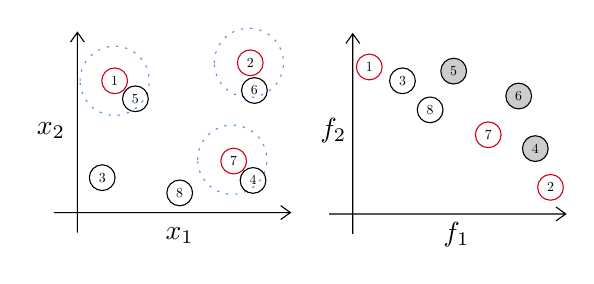
\begin{tikzpicture}[x=0.5pt,y=0.5pt,yscale=-1,xscale=1]
%uncomment if require: \path (0,300); %set diagram left start at 0, and has height of 300

%Shape: Circle [id:dp5136866411017809] 
\draw  [color={rgb, 255:red, 74; green, 144; blue, 226 }  ,draw opacity=1 ][dash pattern={on 0.84pt off 2.51pt}] (69,105) .. controls (69,91.19) and (80.19,80) .. (94,80) .. controls (107.81,80) and (119,91.19) .. (119,105) .. controls (119,118.81) and (107.81,130) .. (94,130) .. controls (80.19,130) and (69,118.81) .. (69,105) -- cycle ;
%Shape: Circle [id:dp3061612047883613] 
\draw  [color={rgb, 255:red, 74; green, 144; blue, 226 }  ,draw opacity=1 ][dash pattern={on 0.84pt off 2.51pt}] (166,92) .. controls (166,78.19) and (177.19,67) .. (191,67) .. controls (204.81,67) and (216,78.19) .. (216,92) .. controls (216,105.81) and (204.81,117) .. (191,117) .. controls (177.19,117) and (166,105.81) .. (166,92) -- cycle ;
%Shape: Axis 2D [id:dp3645341276574614] 
\draw  (50,200.22) -- (221,200.22)(67.1,70) -- (67.1,214.69) (214,195.22) -- (221,200.22) -- (214,205.22) (62.1,77) -- (67.1,70) -- (72.1,77)  ;
%Shape: Circle [id:dp595877391054507] 
\draw  [color={rgb, 255:red, 74; green, 144; blue, 226 }  ,draw opacity=1 ][dash pattern={on 0.84pt off 2.51pt}] (154,162) .. controls (154,148.19) and (165.19,137) .. (179,137) .. controls (192.81,137) and (204,148.19) .. (204,162) .. controls (204,175.81) and (192.81,187) .. (179,187) .. controls (165.19,187) and (154,175.81) .. (154,162) -- cycle ;
%Shape: Axis 2D [id:dp14963900792703488] 
\draw  (249,201.22) -- (420,201.22)(266.1,71) -- (266.1,215.69) (413,196.22) -- (420,201.22) -- (413,206.22) (261.1,78) -- (266.1,71) -- (271.1,78)  ;

% Text Node
\draw  [color={rgb, 255:red, 208; green, 2; blue, 27 }  ,draw opacity=1 ]  (94, 105) circle [x radius= 9.3, y radius= 9.3]   ;
\draw (94,105) node [scale=0.5] [align=left] {1};
% Text Node
\draw  [color={rgb, 255:red, 0; green, 0; blue, 0 }  ,draw opacity=1 ]  (109, 118) circle [x radius= 9.3, y radius= 9.3]   ;
\draw (109,118) node [scale=0.5] [align=left] {5};
% Text Node
\draw  [color={rgb, 255:red, 208; green, 2; blue, 27 }  ,draw opacity=1 ]  (192, 92) circle [x radius= 9.3, y radius= 9.3]   ;
\draw (192,92) node [scale=0.5] [align=left] {2};
% Text Node
\draw    (195, 112) circle [x radius= 9.3, y radius= 9.3]   ;
\draw (195,112) node [scale=0.5] [align=left] {6};
% Text Node
\draw  [color={rgb, 255:red, 208; green, 2; blue, 27 }  ,draw opacity=1 ]  (180, 163) circle [x radius= 9.3, y radius= 9.3]   ;
\draw (180,163) node [scale=0.5] [align=left] {7};
% Text Node
\draw    (194, 177) circle [x radius= 9.3, y radius= 9.3]   ;
\draw (194,177) node [scale=0.5] [align=left] {4};
% Text Node
\draw    (141, 186) circle [x radius= 9.3, y radius= 9.3]   ;
\draw (141,186) node [scale=0.5] [align=left] {8};
% Text Node
\draw    (85, 175) circle [x radius= 9.3, y radius= 9.3]   ;
\draw (85,175) node [scale=0.5] [align=left] {3};
% Text Node
\draw  [color={rgb, 255:red, 208; green, 2; blue, 27 }  ,draw opacity=1 ]  (278, 95) circle [x radius= 9.3, y radius= 9.3]   ;
\draw (278,95) node [scale=0.5] [align=left] {1};
% Text Node
\draw  [color={rgb, 255:red, 0; green, 0; blue, 0 }  ,draw opacity=1 ][fill={rgb, 255:red, 0; green, 0; blue, 0 }  ,fill opacity=0.2 ]  (339, 98) circle [x radius= 9.3, y radius= 9.3]   ;
\draw (339,98) node [scale=0.5] [align=left] {5};
% Text Node
\draw  [color={rgb, 255:red, 208; green, 2; blue, 27 }  ,draw opacity=1 ]  (409, 182) circle [x radius= 9.3, y radius= 9.3]   ;
\draw (409,182) node [scale=0.5] [align=left] {2};
% Text Node
\draw  [fill={rgb, 255:red, 0; green, 0; blue, 0 }  ,fill opacity=0.2 ]  (386, 116) circle [x radius= 9.3, y radius= 9.3]   ;
\draw (386,116) node [scale=0.5] [align=left] {6};
% Text Node
\draw  [color={rgb, 255:red, 208; green, 2; blue, 27 }  ,draw opacity=1 ]  (364, 144) circle [x radius= 9.3, y radius= 9.3]   ;
\draw (364,144) node [scale=0.5] [align=left] {7};
% Text Node
\draw  [fill={rgb, 255:red, 0; green, 0; blue, 0 }  ,fill opacity=0.2 ]  (398, 154) circle [x radius= 9.3, y radius= 9.3]   ;
\draw (398,154) node [scale=0.5] [align=left] {4};
% Text Node
\draw    (322, 126) circle [x radius= 9.3, y radius= 9.3]   ;
\draw (322,126) node [scale=0.5] [align=left] {8};
% Text Node
\draw    (302, 105) circle [x radius= 9.3, y radius= 9.3]   ;
\draw (302,105) node [scale=0.5] [align=left] {3};
% Text Node
\draw (141,217) node   {$x_{1}$};
% Text Node
\draw (48,141) node   {$x_{2}$};
% Text Node
\draw (341,216) node   {$f_{1}$};
% Text Node
\draw (252,141) node   {$f_{2}$};


\end{tikzpicture}


%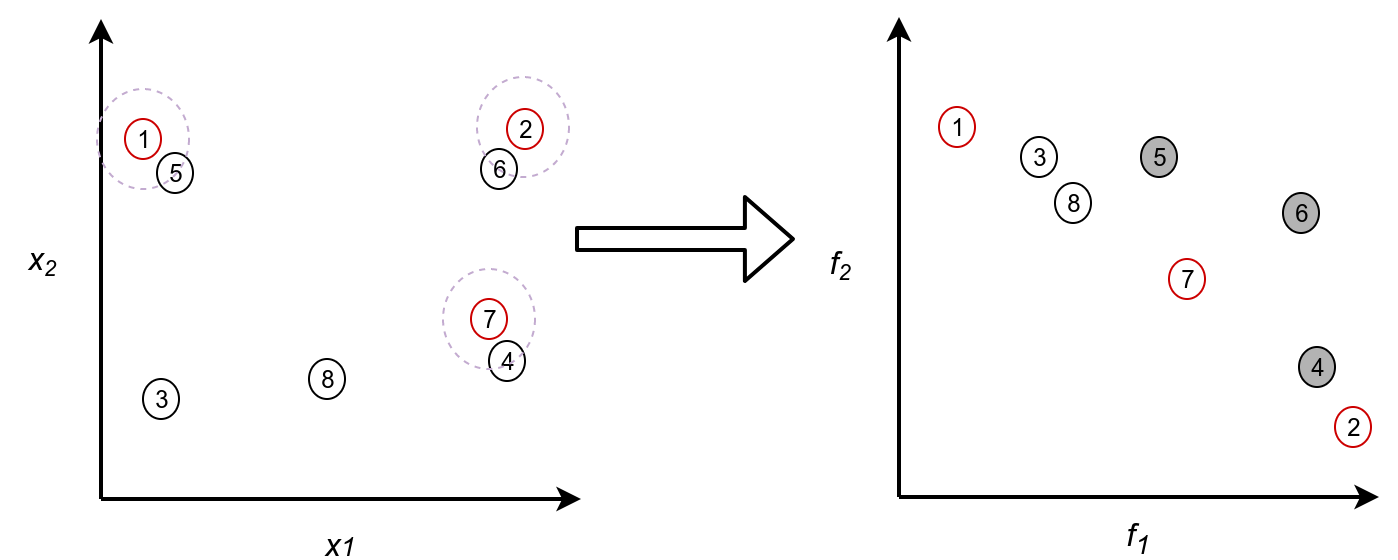
\includegraphics[width=0.45\textwidth]{Images/Fase_Remplazo_2.eps}
\caption{Penalty Method of the Replacement Phase - The left side represents the variables space and the right side the 
objective space}
\label{fig:Hypersphere}
\end{figure}


\subsection{Replacement Phase of VSD-MOEA}

The replacement phase of \EAS{} is in charge of deciding in each generation which are the survivors 
among the members of the previous population and offspring.
%
The novel replacement promotes a gradual movement from exploration to exploitation, which has been a quite i
beneficial principle in the design of single-objective optimizers~\cite{Joel:MULTI_DYNAMIC}.
%
Particularly, the replacement phase operates as follows.
%
First, the members of the previous population and offspring are joined in a multi-set with $2 \times N$ individuals.
%
Then, $N$ individuals must be selected to survive, which is performed with an iterative process that selects an additional
individual at each step.
%
In order to take into account the diversity in the decision space, the Distance to Closest Neighbor (\DCN{}) of each
individual is calculated at each step.
%
Thus, if the multi-set containing the currently selected survivors is called $S$, then the \DCN{} of an individual $I$ is calculated
as $\displaystyle{\min_{s \in S}\ Distance(I, s)}$.
%
Normalized Euclidean distances are considered, so in order to calculate distances between any two individual $A$ and $B$, 
Eq. (\ref{eqn:distance}) is applied.
%
\begin{equation}\label{eqn:distance}
Distance(A, B) =   \left ( \frac{1}{n}  \sum_{i=1}^n \left ( \frac{A_i - B_i}{x_i^{(U)} - x_i^{(L)}} \right )^2  \right)^{1/2}
\end{equation}

Note that individuals with large \DCN{} values contribute significantly to promote exploration.
%
In order to avoid an excessive decrease of the exploration degree, individuals with a \DCN{} value lower 
than a threshold value are penalized and they can only be selected if non-penalized individuals do not exist.
%
Then, among the non-penalized individuals, an objective-space density estimator is used to select the additional
survivor of the iteration.
%
In our case, the novel density estimator described in the next subsection is used. 

In order to better visualize the penalty method, it can be considered that after selecting each survivor, a hyper-sphere 
centered in such candidate solution --- in the variable space --- is created.
%
Then, all the individuals that are inside a hyper-sphere are penalized and the objective-space estimator takes 
into account only the non-penalized individuals.
%
This is illustrated in Fig.~\ref{fig:Hypersphere}, which represents a state where three individuals have been 
selected to survive and an additional survivor must be picked up.
%
The left side shows individuals in the variable space.
%
Current survivors are marked with a red border and each one of them is surrounded by a blue dash circle with 
radius $D_t$.
%
In this situation, the penalized individuals are the number 4, 5, and 6.
%
In the objective space ---right side --- penalized individuals are shown with gray background, indicating
that the objective-space density estimator can not select them.

Since penalizing with a large threshold value --- radius of the hyperspheres --- induces a higher degree of 
exploration, it makes sense to reduce this value during the optimization process.
%
This is precisely one of the keys of our proposal.
%
The sizes of the hyper-spheres are modified dynamically by taking into account the stopping 
criterion and elapsed generations.
%
Particularly, the radius is decreased in a linear way starting from an initial distance.
%
This means that in the initial phases exploration is promoted.
%
However, as the size of the radius decreases only very close individuals are penalized, meaning that more 
exploitation is performed.
%
Note that this method requires a parameter which is the initial radius of the hyper-spheres which is denoted as $D_I$. 
%
Setting this parameter with a large value might provoke the penalization of a lot of individuals, 
thus non-useful diversity might be maintained.
%
However, too small values might not prevent fast convergence and therefore the approach with such a parameterization 
might behave as a traditional non-diversity based approach.
%
The robustness of the proposal with respect to this additional parameter is studied in our experimental validation.

\begin{algorithm}[t]
\algsetup{linenosize=\tiny}
  \scriptsize
	\caption{Replacement Phase of VSD-MOEA} 
\begin{algorithmic}[1]
\STATE Input: $P_t$ (Population of current generation), $Q_t$ (Offspring of current Generation)
    	\STATE Output: $P_{t+1}$ 
        \STATE $R_t = P_t \cup Q_t$ \label{alg:1}
        \STATE $P_{t+1} = \emptyset$ \label{alg:2}
        \STATE $Penalized = \emptyset$ \label{alg:3}
				\STATE $D_t = D_I - D_I * \frac{G_{Elapsed}}{0.9*G_{End}}$ \label{alg:4}
				\FOR{$k \in {1...M}$}
					\STATE Move to $P_{t+1}$ the individual that optimize $AWF_k$ (Eq.~\ref{eqn:extremes})
				\ENDFOR
        \WHILE{ $|P_{t+1}|$ $\leq$ N } \label{alg:6}
					\STATE Compute $DCN$ of individuals in $R_t$ with $P_{t+1}$ used as reference set \label{alg:7}
					\STATE Move to $Penalized$ the individuals in $R_t$ with $DCN < D_t$  \label{alg:8}
        	\IF{$R_t$ is empty} \label{alg:9}
						\STATE Compute $DCN$ of individuals in $Penalized$ with $P_{t+1}$ used as reference set \label{alg:10}
						\STATE Move to $R_t$ the individual in $R_t$ with largest $DCN$ \label{alg:11}
        	\ENDIF
					\STATE $non-dominated-rank-assignment(R_t \cup P_{t+1}) $ \label{alg:12}
					\STATE Use the novel density estimator to select a new survivor from $R_t$ and move it to $P_{t+1}$\label{alg:13}
        \ENDWHILE
    	\RETURN $P_{t+1}$ \label{alg:14}
	\end{algorithmic}
\label{alg:Replacement_Phase}
\end{algorithm}


Algorithm~\ref{alg:Replacement_Phase} fully describes the replacement phase of \VSDMOEA{}.
%
First, the population of the previous generation ($P_t$) and the offspring ($Q_t$) are joined
in $R_t$ (line \ref{alg:1}).
%
The multiset $R_t$ contains, in each iteration, the remaining non-penalized individuals that might be selected 
to survive.
%
The population of survivors ($P_{t+1}$) and the set containing the penalized individuals are initialized to
the empty set (lines \ref{alg:2} and \ref{alg:3}).
%
Then, the threshold value ($D_t$) that is used to penalize too close individuals is calculated (line \ref{alg:4}).
%
Note that $D_I$ denotes the initial radius or threshold value, $G_{Elapsed}$ is the amount of generations that have 
been evolved, and $G_{End}$ is the stopping criterion, i.e. the number of generations that are to be evolved 
in the execution of \VSDMOEA{}.
%
The linear decrease is calculated so that after the $90\%$ of the generations, the $D_t$ value is lower than 0, 
meaning that no penalties are performed.
%
This means that in the first $90\%$ of the generations, more exploration than in traditional \MOEAS{} is induced, 
whereas in the final stages, a traditional \MOEA{} is applied.
%
Finally, for each objective a hiqh-quality candidate solution is selected to survive.
%
Note that selecting the best solution for each objective might provoke some drawbacks realated to accepting small improvement
in an objective at the cost of important worsening in other objectives~\cite{deb2016optimality}.
%
To solve this issue augmented functions can be applied, which has been the alternative used in this paper.
%
Particularly, for each objective $k$, the candidate solution that minimizes the Augmented Weighted Function (AWF)
given in Eq.~\ref{eqn:extremes} is selected and consequently moved to $P_{t+1}$ (line~\ref{alg:5}).
%
Note that, augmented functions usually take into account weight vectors with the aim of dealing with objectives
that present very different scales.
%
Since benchmarks that have similar scales in each objective have been used in this paper, there was no need to apply
such weight vectors.

\begin{equation}\label{eqn:extremes}
AWF_k (\vec{x}) = f_k(\vec{x}) + 10^{-4} \times  \sum_{j=1}^m f_j( \vec{x} )
\end{equation}


Then, an iterative process that selects an individual at each iteration is executed until the survivors
set contains $N$ individuals (line \ref{alg:6}).
%
The iterative process works as follows.
%
First, the \DCN{} value of each reamining non-penalized individual is calculated (line \ref{alg:7}).
%
Then, those individuals with a \DCN{} value lower than $D_t$ are moved to the set of penalized individuals (line \ref{alg:8}).
%
If all the remaining individuals are penalized (line \ref{alg:9}), it means that the amount of exploration is lower than expected.
%
Thus, the individual with largest \DCN{} values is recovered, i.e. moved to the non-penalized individuals 
set (lines \ref{alg:10} and \ref{alg:11}).
%
Finally, the objective space is taken into account.
%
Specifically, the candidate individuals and the current survivors are joined.
%
Then, the \textit{fast-non-dominated-sort} procedure is executed with such a set, stopping as soon as a front with 
a candidate individual is found (line \ref{alg:12}).
%
Then, for each candidate individual that belongs to the lowest front, the individual with higher contribution to 
the diversity in the objective space is selected (line \ref{alg:13}).
%
The specific way in which the diversity in the objective space is measured is described in the next section.
%

%Note also that, as part of the diversity calculation of the variable space, a metric should be selected.
%
%Since our experimental validation is performed with a continuous domain, the normalized Euclidean distance is used.
%%
%However, in discrete domains other distance metrics such as the Manhattan, or the Hamming distance might be considered, and the definition of
%such distance might affect the performance of the approach~\cite{Segura:17}.


%The main idea of replacement phase dwell in compute the contribution by each individual to diversity  in both spaces.
%
%Hence in each iteration just one individual is selected as survivor until the size of population is reached.
%
%Consequently this methodology separate the suitable candidates based in diversity of the variable space, afterward the best candidate in objective space is selected.
%

%
%The figure \ref{fig:Hypersphere} shows one iteration of the Replacement Phase where the reference individuals are $\{1, 2, 7\}$ and candidate individuals are $\{3, 4, 5, 6, 8\}$. 
%
%The individuals $\{4, 5, 6\}$ are moved to penalized set, since that each one is inside of a hypersphere (gray dotted circles) related to a reference individual.
%
%Finally, the candidate solutions are $\{2, 8\}$, due that both belongs to the same rank, the solution $8$ is selected since it has a better contribution to the diversity in the objective space.

%
%
%
%
% %The function definitions from algorithm~\ref{alg:Replacement_Phase} are explained as follow:
% %
% \begin{itemize}
% \item Diversity\_Variable\_Space(A,B): for each individual from set A an euclidean distance is computed in variable space to the closest solution from the set B.
% \item Diversity\_Objective\_Space(A,B): for each individual from set A an euclidean distance is computed in objective space to the closest solution from the set B.
%\end{itemize}
%
%
%

%ESto hay que moverlo a Experimental Validation
%Due that the initial diversity is influenced by  $D_I$ parameter, several experiments with different values have been realized.
%
%Accordingly that each dimension is normalized in the unity, the maximal hypersphere of the variable decisions is denoted by $\sqrt{N}$ where $N$ is the dimension of the variable space. 
%
%Under those circumstances, the hypersphere with radius $\sqrt{N}$ will cover outside from the bounds, for this reason it is multiplied by a factor $k$  resulting in the formula$D_I = k * \sqrt[]{N}  \rightarrow k \in (0,1)$.
%
%Empirically, the ideal configuration that provides quality solutions is $k=0.25$ .
%
%Additionally, the algorithm empirically is enough stable, given that different values of $k$ does not provide drastically differences in the solutions.

\subsection{A Novel Density Estimator for the Objective Space}
\label{subsection:density}

Since the dominance definition is not related to the preservation of diversity in the objective space,
dominance-based \MOEAS{} incorporate special procedures to maintain diverse solutions, such as clustering and/or crowding.
%
In this paper, we define a novel distance metric, and an iterative heuristic selection approach, which selects an individual of the best front and with the largest defined distance.
%
Specifically, the novel distance is called ``Improvement Distance'' (ID) and it 
follows the same principles that guided the design of both indicators the IGD+ and $I_{\epsilon +}$~\cite{Joel:Inverted_Generational_Distance_Plus}, \cite{Joel:IBEA}, \cite{zitzler2003performance}.
%
The main idea is to prefer those individuals whose quality in all objectives is similarly preserved.
%
Particularly, a non-dominated individual can be very distant to the Pareto Front due that such individual could be the best in one objective but mainly deteriorated in the rest of objectives, so as result it has high diversity in objective space.
%----
%The key idea is that, a direct Euclidean distance is used, those individuals that have very high values in some
%of the objectives might present very large distances which is not an adequate property.
%
In fact, high improvements in one objective value are related to larger selection probabilities and not the opposite, so this behavior should be avoided.
%
%In order to take this principle into account, when calculating the distance between two individuals

The key idea takes into account the dominance relation between the candidate and reference individuals. % when the distance is computed.
%
%
Consequently, the reference and the candidate individuals are compared.
%
If the reference individual is dominated by the candidate individual, then the euclidean distance with no modification is implemented.
%
However if they are non-dominated with each other, then is calculated the minimum distance from the reference individual to the dominated region by the candidate individual. %
%
Additionally, if the candidate individual is dominated by the reference individual, then is computed the $I_\epsilon$ indicator, that gives the minimum distance by which the candidate individual needs to or can be translated in each dimension in objective space such that the reference individual is dominated.
%
Therefore, this distance can be viewed as an amount of inferiority of the solution in comparison with the reference individual.	
%
The improvement distance is defined in Equation (\ref{eq:ImprovementDistance}) which incorporates the $I_\epsilon$ indicator (Equation \ref{eqn:epsilonindicator})  where $R$ and $C$ are the reference and candidate solutions respectively. 
\begin{equation} \label{eq:ImprovementDistance}
\begin{split}
 ID(R, C) = &  \left (\sum_{i=1}^M \left (max(0, R_i - C_i \right ))^2  \right)^{1/2} - I_\epsilon(R,C) \\
% &I_\epsilon(R,C) = min_{\epsilon} \{ f_i(C) - \epsilon \leq f_i (R) \quad \forall i \in \{1,..,m \} \}
\end{split}
\end{equation}
\begin{equation}\label{eqn:epsilonindicator}
\begin{split}
I_\epsilon(R,C) = \begin{dcases}
   min_{\epsilon} \{ f_i(C) - \epsilon \leq f_i (R) \} \} & R \preceq C \\
%\quad \forall i \in \{1,..,m \} \\
    0 & otherwise
	\end{dcases}
\end{split}
\end{equation}

Specifically, this distance is considered as a Weakly Pareto Compliant Indicator.
%
In addition, this metric relaxes some difficulties encountered when the number of objectives is increased, given that the solutions in many objectives are usually non-dominated with each other by using the Pareto dominance relation.
%
This means a very low selection pressure toward the Pareto front in Pareto-dominance-based MOEAS \cite{Joel:Optimization_Of_Scalarizing_Functions_Through_Evolutionary_MOEAS}.
%
Principally, the improvement distance is effective with over-prioritization  of dominance-resist solutions i.e., solutions with exceptional performance in one objective and extremely poor performance in many others \cite{Joel:Failure_MOEAs}.
%

Given that the design of this MOEA is considered for long-term executions, the algorithm \ref{alg:Replacement_Phase} is implemented efficiently.
%
Thus, the distances are pre-computed and are updated in each iteration, the same for the dominance count information that is used in the \textit{conditionally-non-dominated-sort}.
%
In fact, the worst case complexity of this algorithm is $O((3 N)^2 \times n)$, since that the dimension of the decision variable space is usually bigger than the number of objectives. 



\section{Multimedia Material}
This section is devoted to provide a detailed description of the included video \footnote{Alternatively, the video can be consulted in this link \url{https://www.youtube.com/watch?v=ElxK_95n4lE&feature=youtu.be}}.
%
Specifically, to have a better understanding of the behaviour of each algorithm with the WFG5 problem a simulation is recorded.
%
The WFG5 problem is selected given its properties being perhaps the most difficult one --under standard parameterization-- of the WFG problems.
%
The main peculiarity of this problem dwell in its desceptiveness, which involves several local optimal regions that mislead the search process of the algorithms.
%
Principally, the Pareto geometry of this problem is convex, and such Pareto optimal solutions of the distance parameters have the following values:
%
\begin{equation}
   x_{i=k+1:n} = 2i \times 0.35
\end{equation}
Therefore, in this simulation is taken into account the standard parameterization indicated in the main document, as well the specified configuration.
%
Each algorithm was run with two objectives and two decision variables, whose number of position and distance parameters was set to one, and the number of generations was set to $1000$.
%

The video is vertically divided in two sides, the left-side and right-side representing each one the objective space and the decision variable space respectively.
%
In the decision variable space (right-side) each local optimal region is remarked with a horizontal blue line, and the global optimal region is remarked with a horizontal red line.
%
Particularly, the position and distance parameters are denoted by $x_1$ and $x_2$ respectively.
%
The video shows that after ten generations the state-of-the-art-MOEAs have converged prematurely to the local optimal regions, contrarely to the VSD-MOEA which is still exploring.
%
Approximatelly on the $30\%$ of total generations, VSD-MOEA has found three individuals in the global optimal region, and few generations before (in the $40\%$) has located several individuals around the optimal region.
%
At the $50\%$ of total generations, VSD-MOEA has converged to the optimal region (red horizontal line) avoiding the remaining sub-optimals (blue horizontal lines).
%
Finally, the remaining $50\%$ of generations VSD-MOEA keeps improving quality in the objective space.

%%Figures ONE TWO THREE, are taken of the video and belong to the 0\%, 50\% and 100\% of total generations.
%%
%%\begin{figure}[t]
%%\centering
%%\begin{tabular}{l}
%% 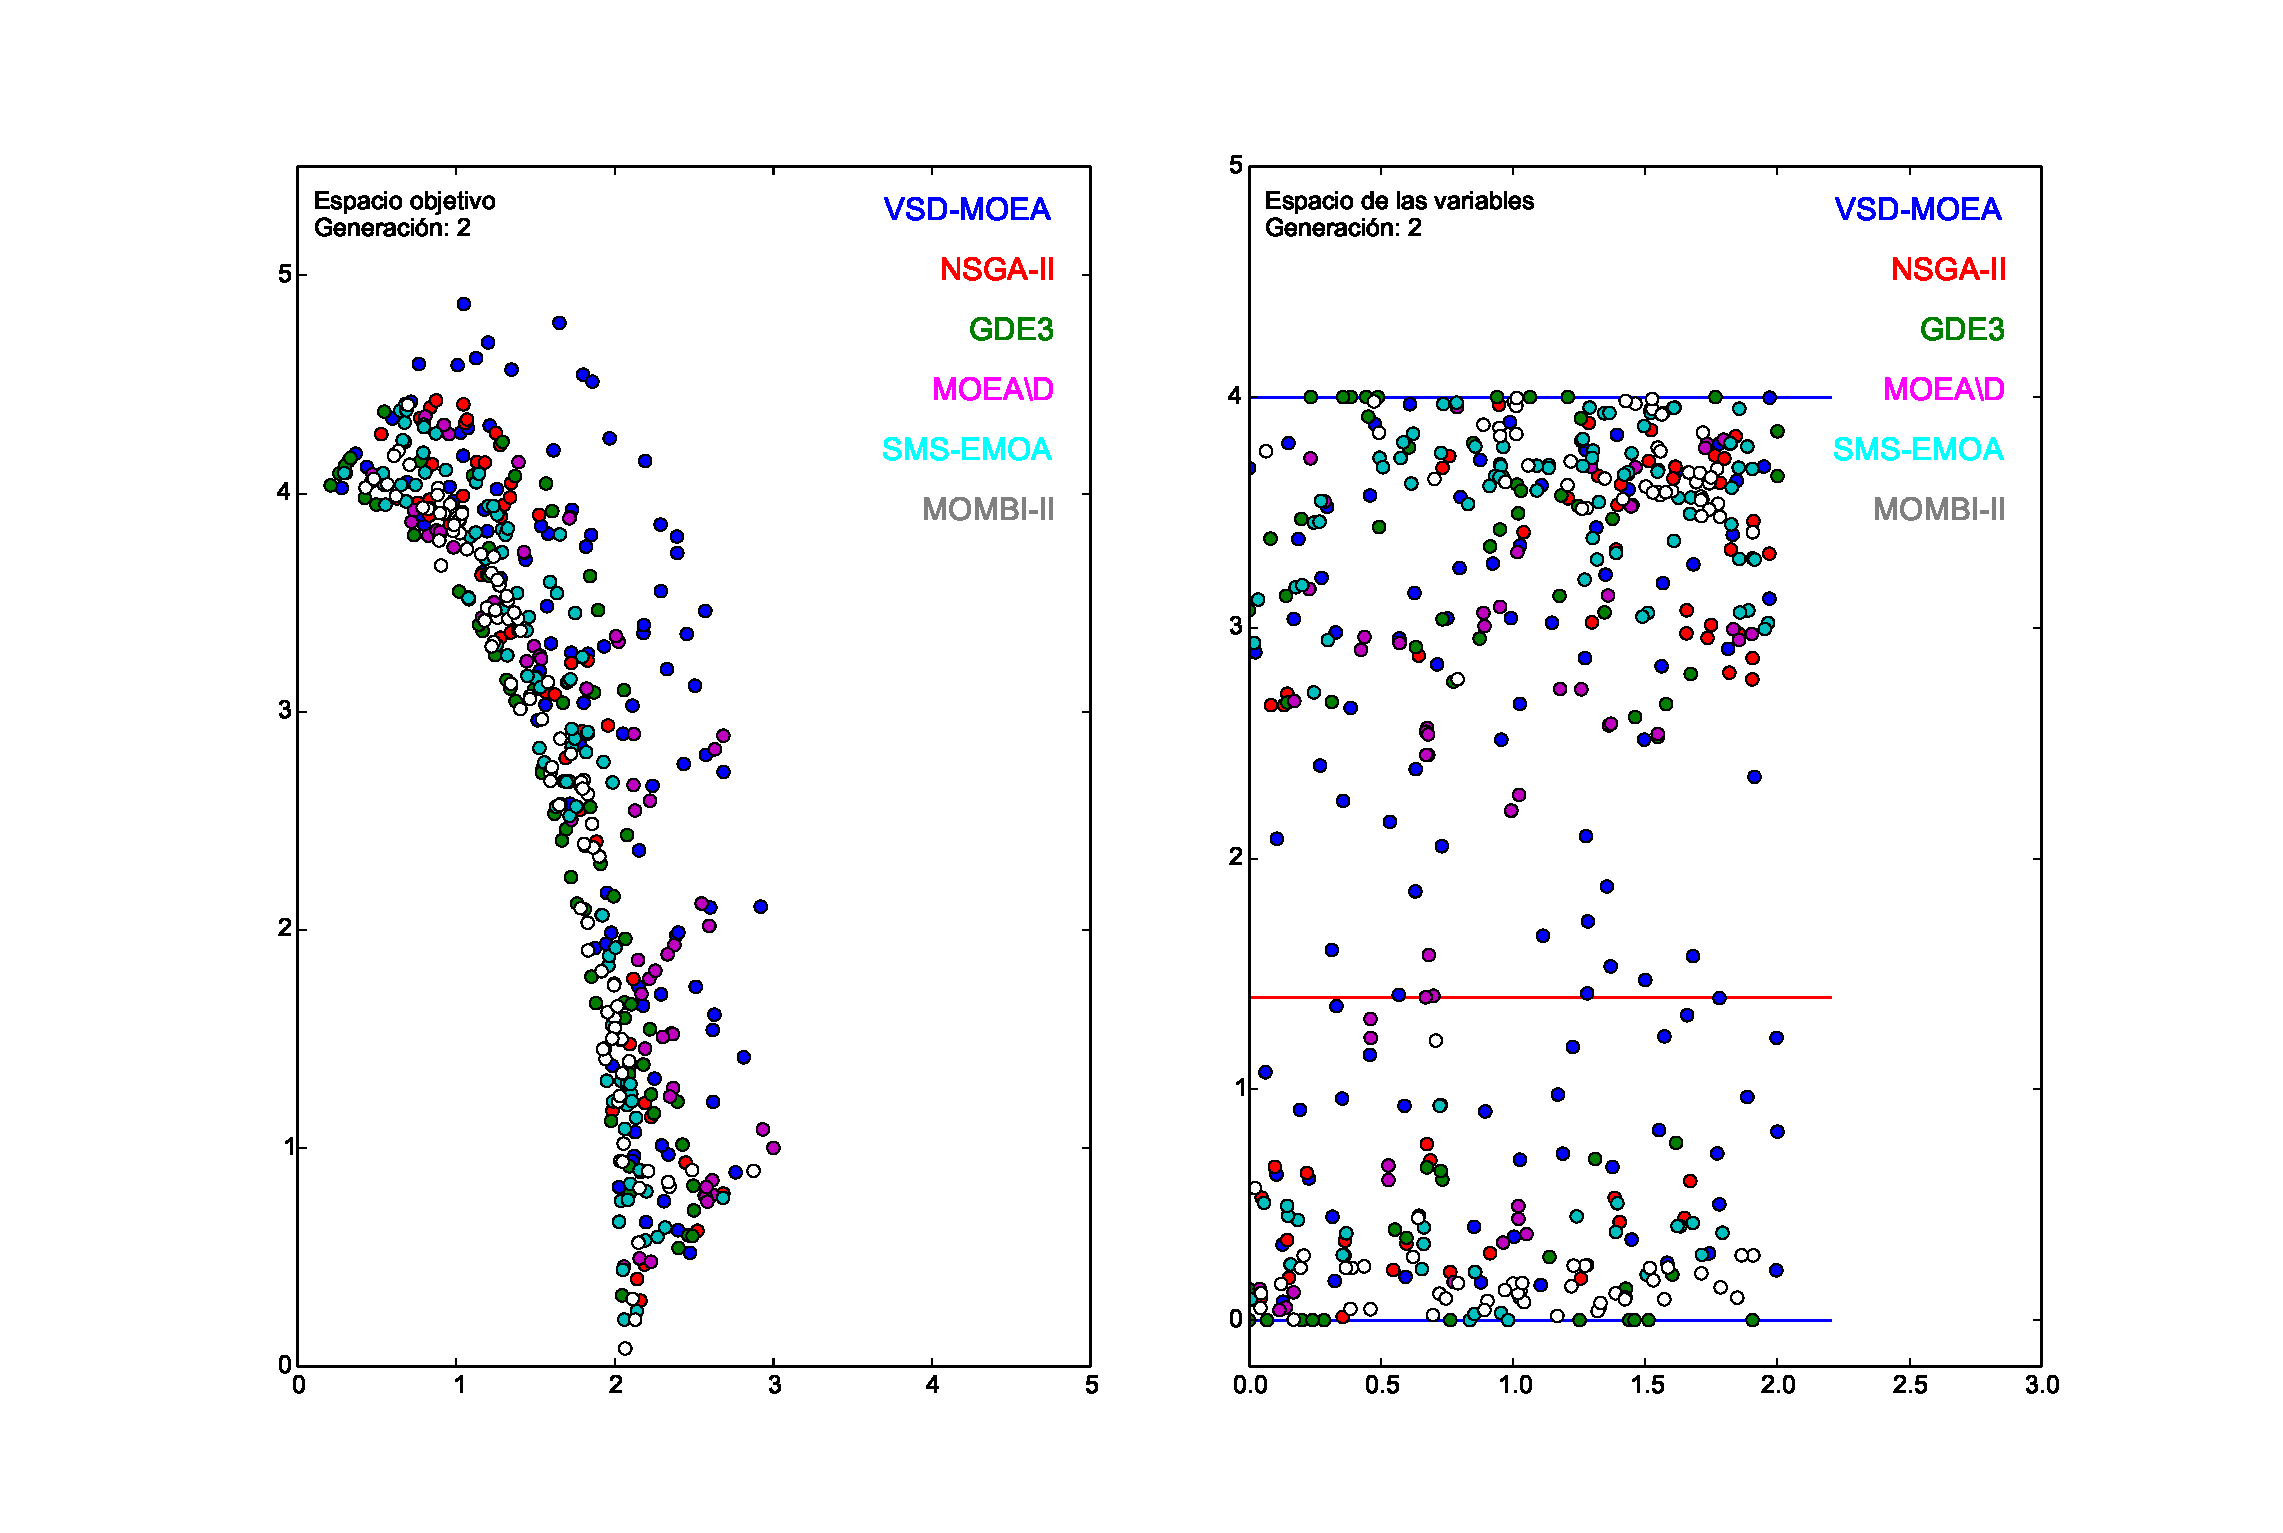
\includegraphics[scale=0.3]{Images/Simulacion_Algoritmo_1.eps}\\[0cm]%[-0.14cm] 
%% 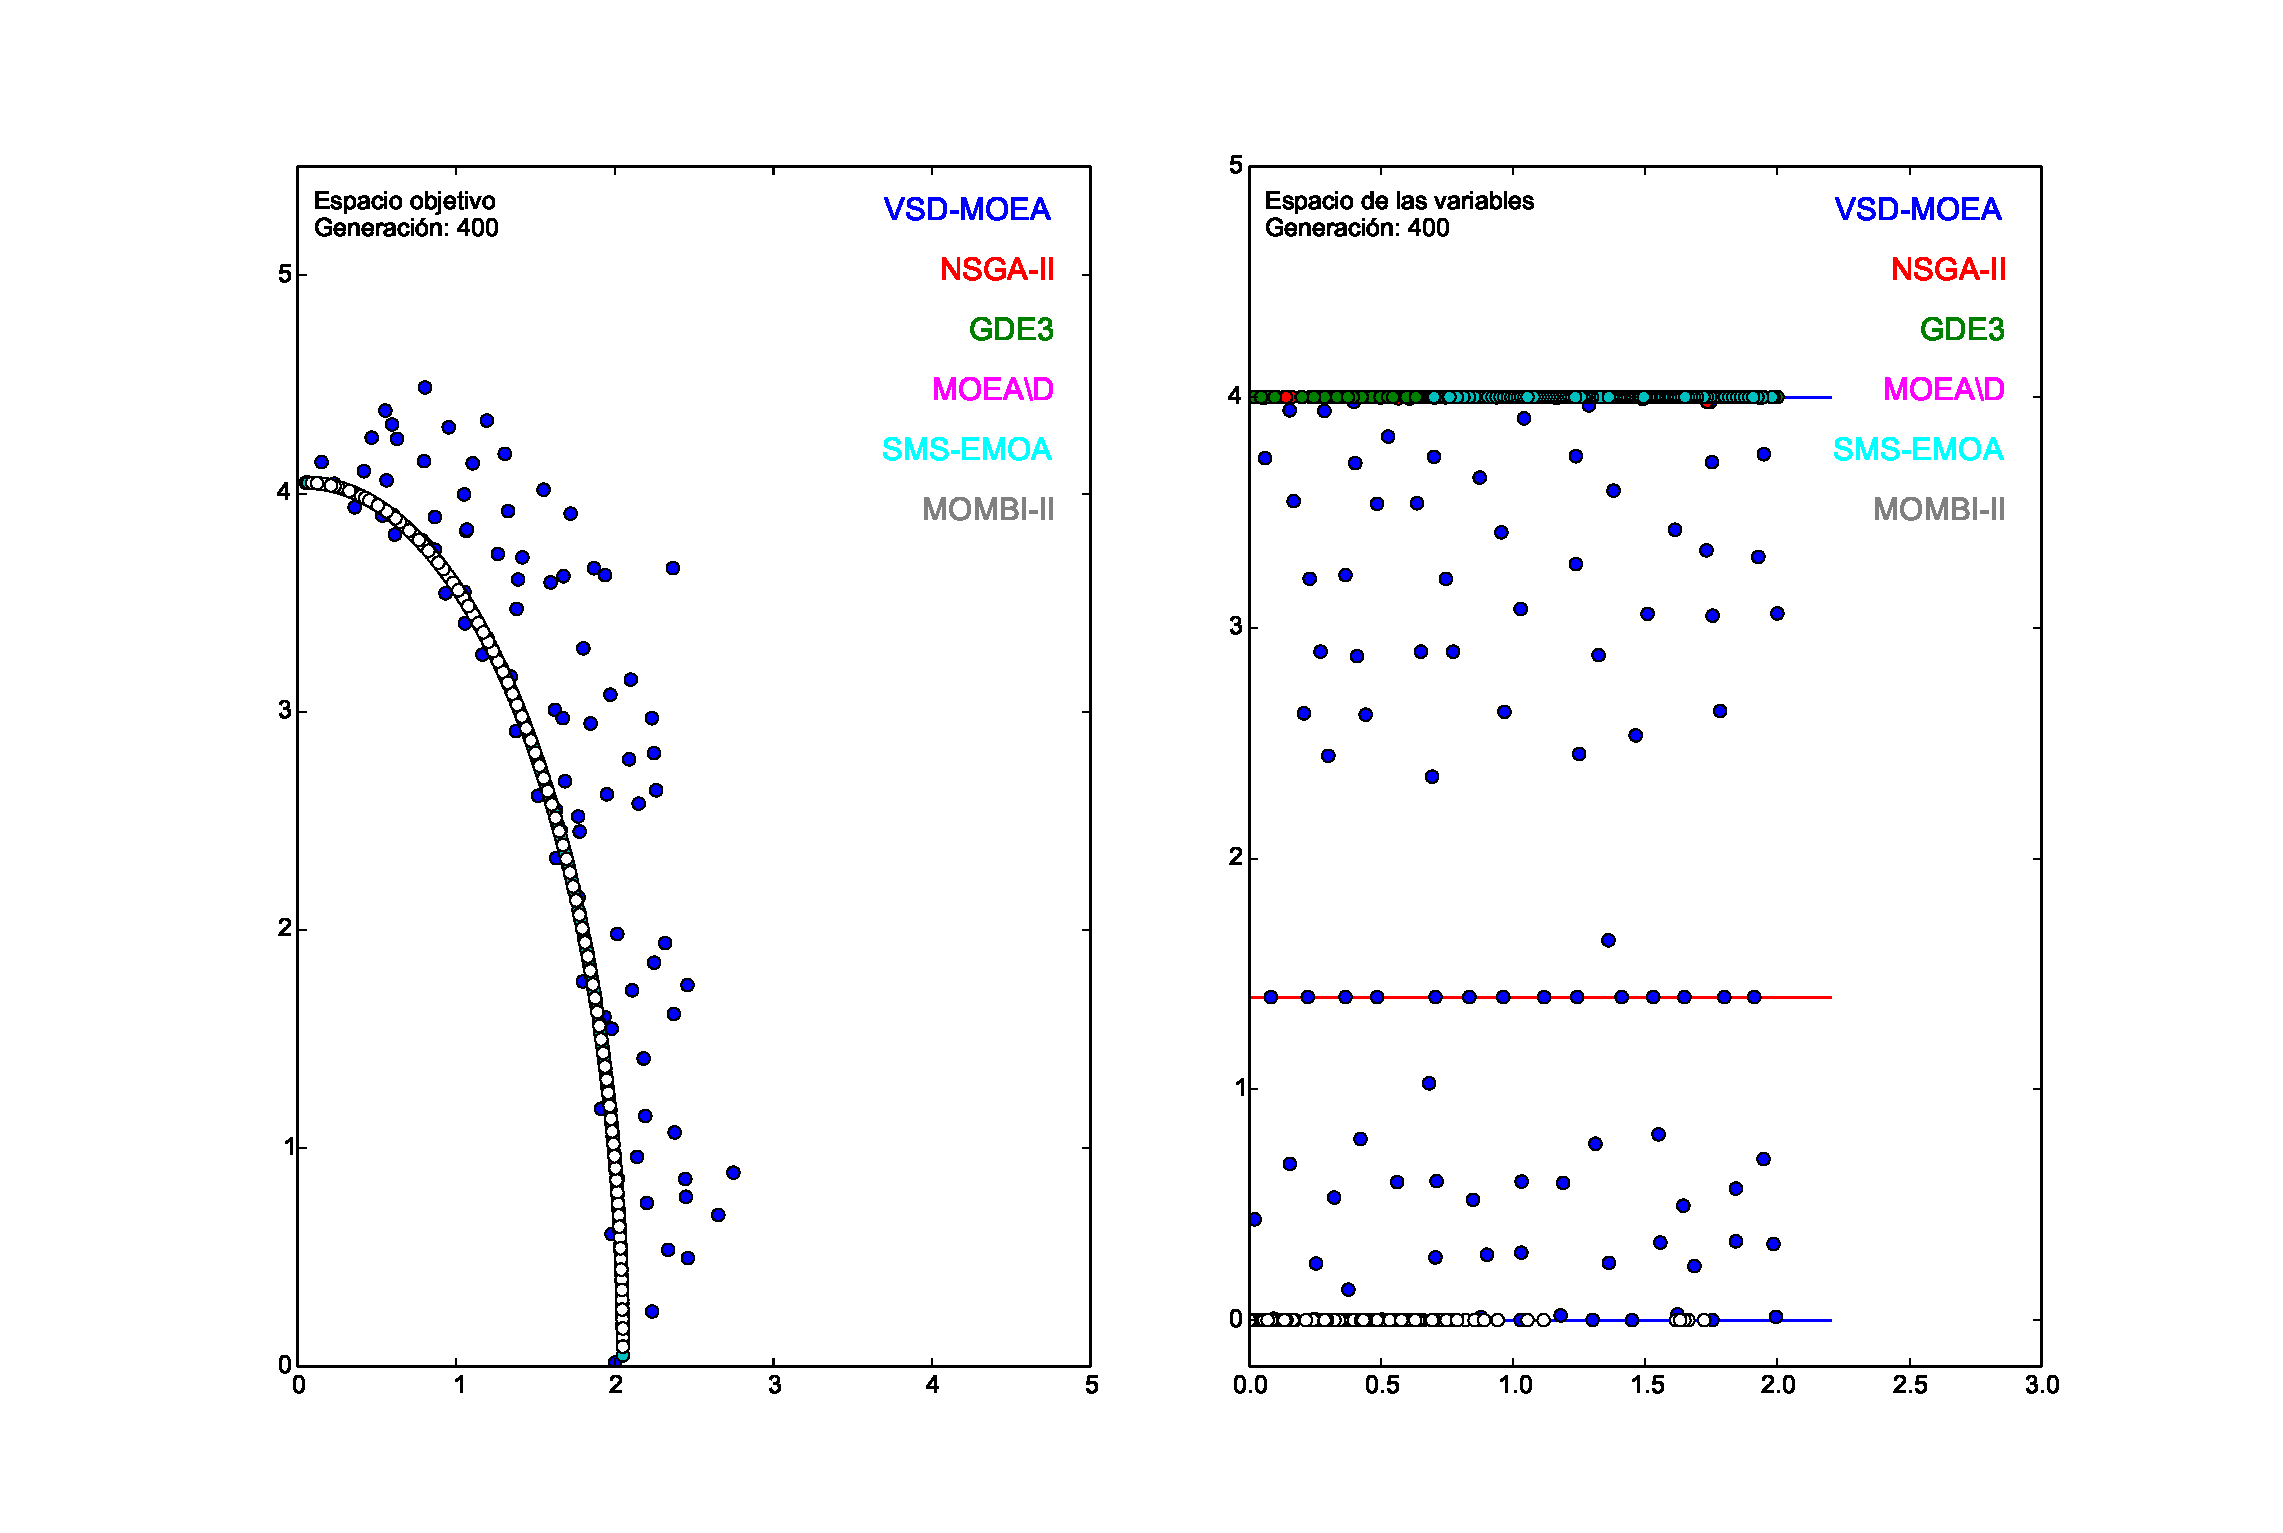
\includegraphics[scale=0.3]{Images/Simulacion_Algoritmo_4.eps}\\[0cm]%[-0.14cm] 
%% 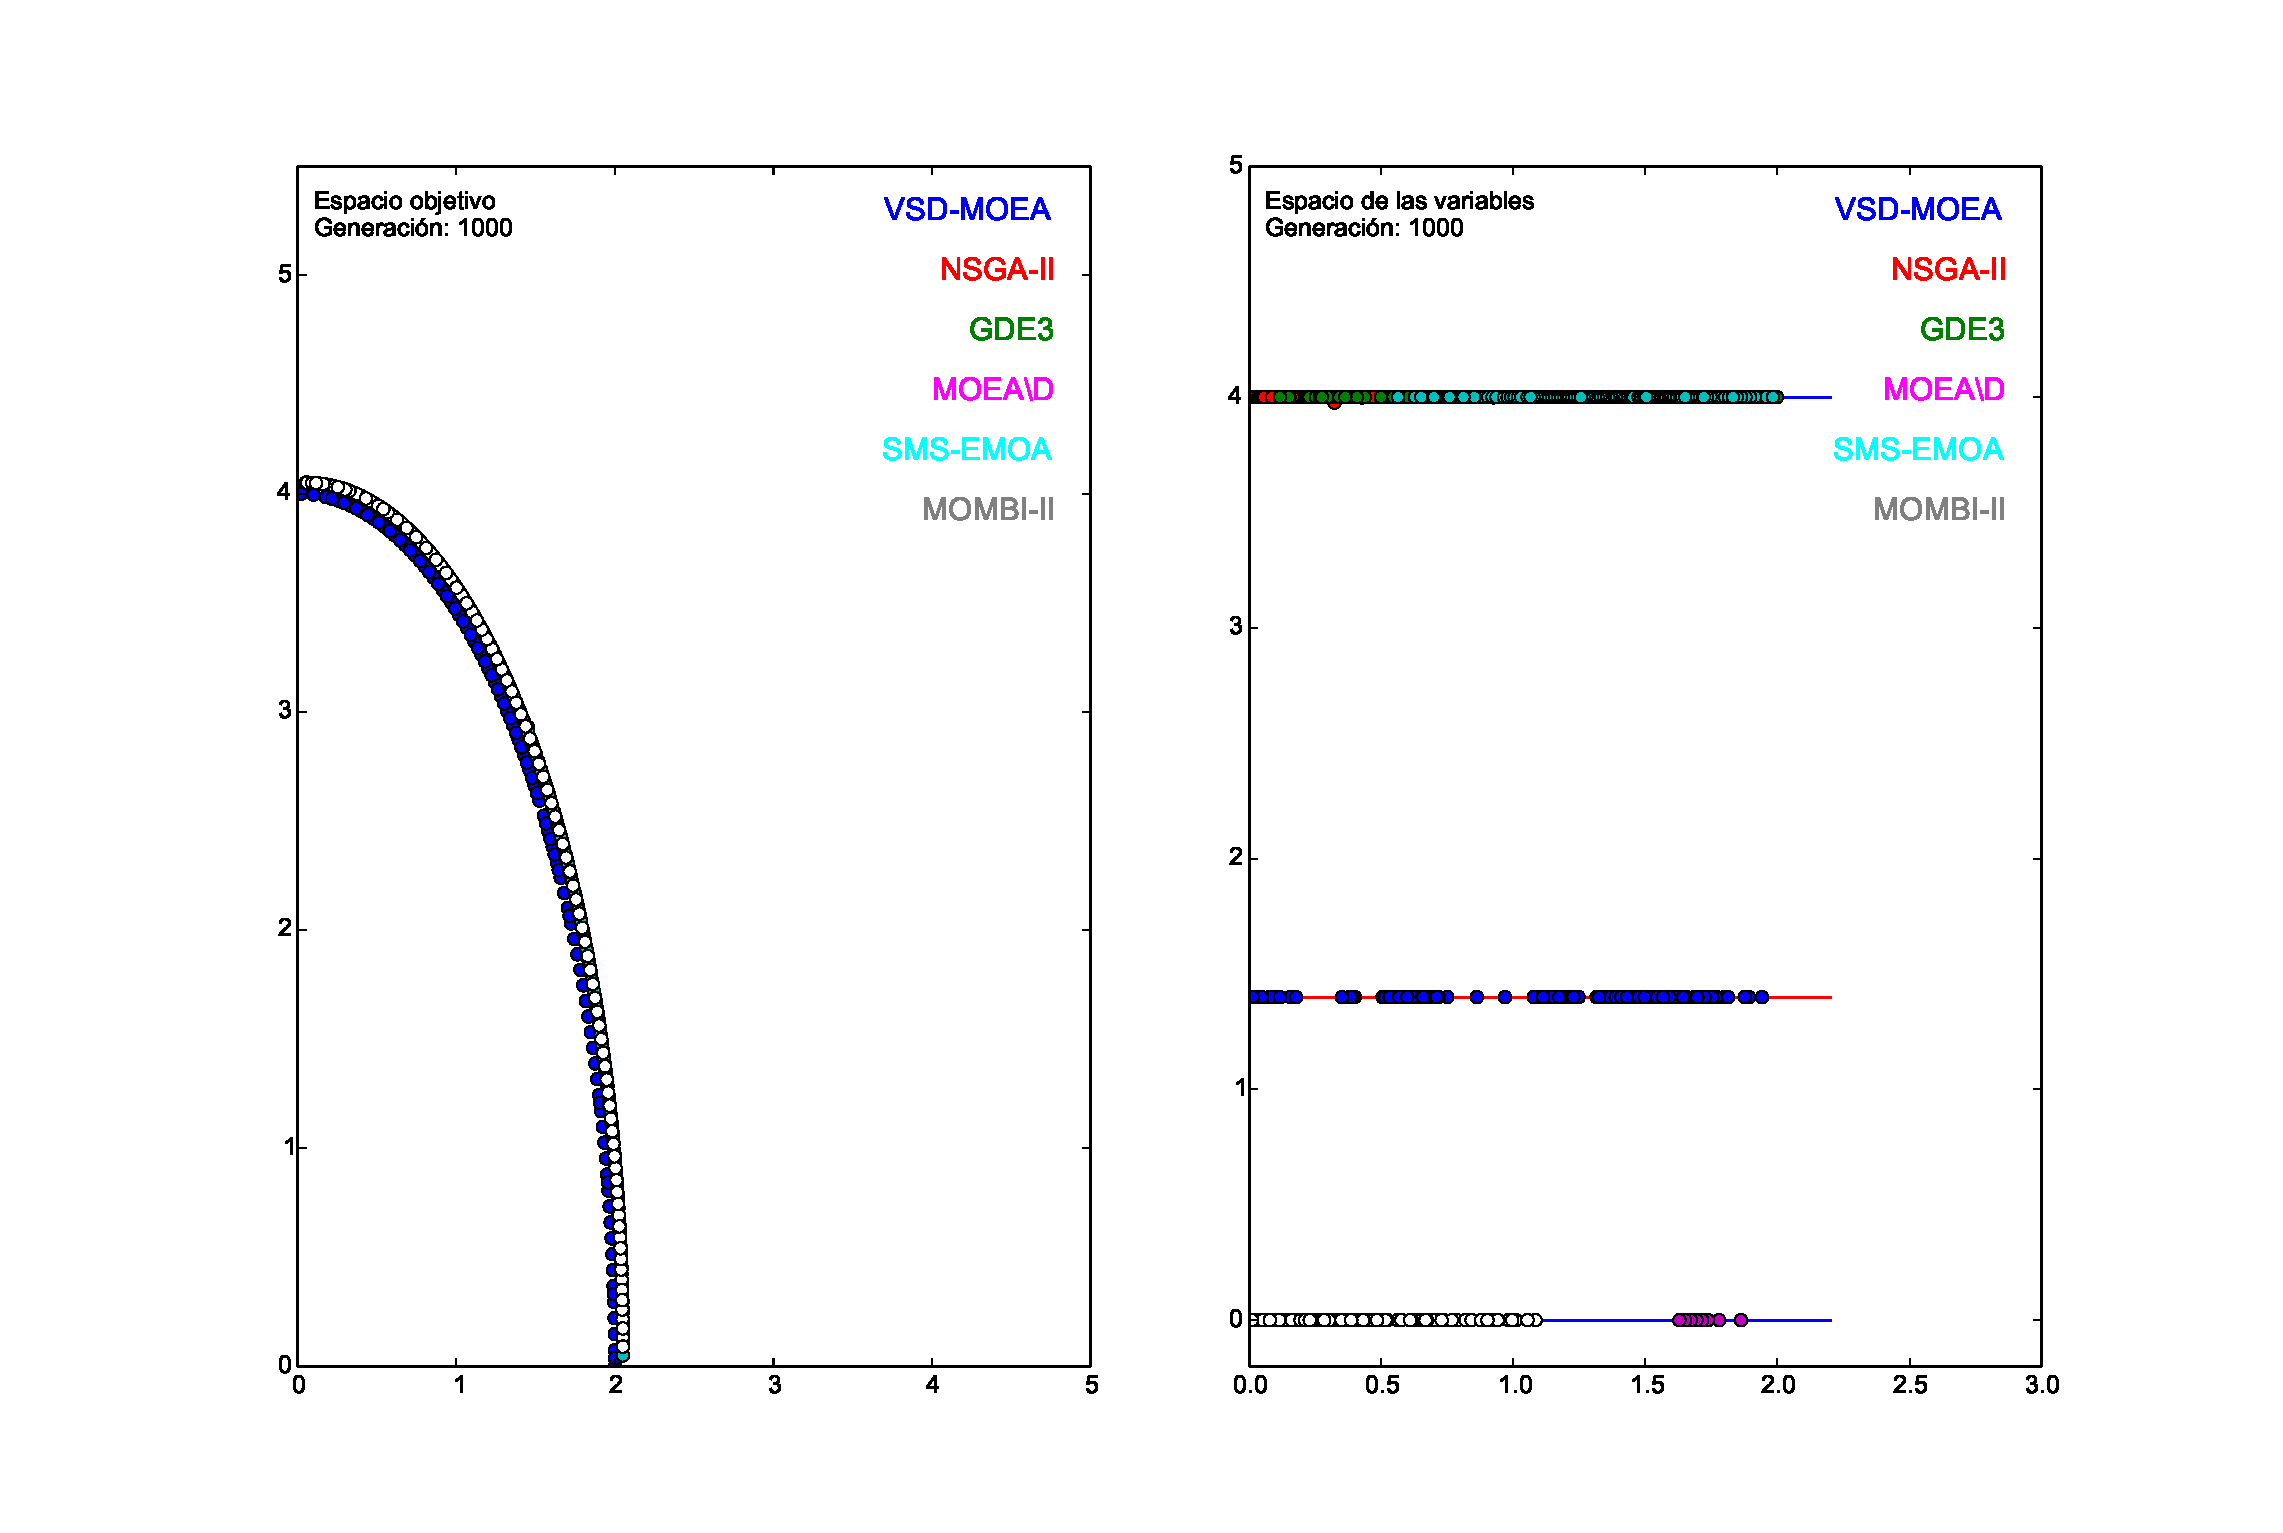
\includegraphics[scale=0.3]{Images/Simulacion_Algoritmo_5.eps}\\[0cm]%[-0.14cm] 
%%\end{tabular}
%%\caption{Performance of \MOEAS{} for the problems with three objectives considering three ranges of stopping criterion: short-term (first row), middle-term (second row) and long-term (third row).}\label{fig:Performance_time_3obj}
%%\end{figure}


\section{Experimental Validation}
In this section the statistical and test results of the IGD+ are shown \cite{Joel:Inverted_Generational_Distance_Plus}.
%
Particularly, the stopping criterion was set to $250,000$ generations.
%
Table \ref{tab:StatisticsIGDP_2obj} shows the attained IGD+ for the benchmark functions with two objectives.
%
Especifically, the minimum, maximum, mean and standard deviation of the IGD+ for each tested method and function is presented.
%
The last row shows the results considering all the functions together.
%
In each function, the data of the method that attained the largest mean is shown in bold face.
%
Additionally, all the methods that are not statistically inferior than such method are shown in bold face.
%
Thus, the methods shown in bold face in a give problem are referred to as the winning methods.
%
Therefore, the amount of functions where each method attained the best results with two objectives are VSD-MOEA and R2-EMOA with 8 and 13 respectively.
%
Evenmore, the mean IGD+ of all the function attained by the VSD-MOEA is quite superior than the remaining algorithms (including the R2-EMOA).
%
In fact, the total mean of R2-EMOA ($0.060$), NSGA-II ($0.051$) and MOEA/D ($0.062$) are similar.
%
In contrast VSD-MOEA achieved a better value ($0.021$).
%
Futhermore, in the cases where VSD-MOEA loses, the difference with respect to the best methods is not large.
%
In fact, the IGD+ attained by VSD-MOEA and by the best method was never larger than $0.05$.
%
However, all the other methods presented a deterioration larger than $0.05$ in several cases.
%
The counting of functions with deterioration larger than $0.05$ is $7$, $5$ and $8$ for MOEA/D, NSGA-II and R2-EMOA respectively.
%
Therefore, if VSD-MOEA loses in some cases, its deterioration is always small resulting in a robust behavior.

In order to have a better understading, several pair-wise statistical tests were done among each tested method in each function.
%
As it is explained in the main document, the table~\ref{tab:Tests_IGDP_2obj} shows statistical test for the two-objective cases.
%
The calculated data confirms that although VSD-MOEA loses in some cases, the overall numbers of wins and losses favor VSD-MOEA.
%

Tables~\ref{tab:StatisticsIGDP_3obj} and~\ref{tab:Tests_IGDP_3obj} shows the same information for the problems conformed of three objectives.
%
In this case, the superiority of VSD-MOEA is even clearer.
%
Takng into account the mean of all functions, VSD-MOEA attained much larger mean of the IGD+ in comparison to the other methods.
%
Particularly, VSD-MOEA attained the value $0.059$, whereas the second ranked algorithm (R2-EMOA) attained a value $0.093$.
%
The difference between IGD+ attained by VSD-MOEA was never larger than $0.05$.
%
However, all the other methods presented a deterioration larger than $0.05$ in at least one problem.
%
Particularly, it happened in $5$, $8$ and $7$ problems for MOEA/D, NSGA-II and R2-EMOA respectively.
%
Evemore, VSD-MOEA is notably superior than the other methods in terms of both: total deterioration and statistical-tests (wins).
%
VSD-MOEA won in $49$ pair-wise comparisons, whereas the second best ranked algorithm (R2-EMOA) won in $35$ pair-wise comparisons.



% Please add the following required packages to your document preamble:
% \usepackage{graphicx}
\begin{table*}[t]
\centering
\caption{Statistics IGD+ with two objectives}
\label{tab:StatisticsIGDP_2obj}
%\resizebox{\textwidth}{!}{%
\begin{tabular}{cc|c|c|c|c|c|c|c|c|c|c|c|c|c|c|c}
\cline{2-17}
 & \multicolumn{4}{c|}{\textbf{MOEA/D}} & \multicolumn{4}{c|}{\textbf{NSGA-II}} & \multicolumn{4}{c|}{\textbf{R2-EMOA}} & \multicolumn{4}{c}{\textbf{VSD-MOEA}} \\ \cline{2-17} 
 & \textbf{Min} & \textbf{Max} & \textbf{Mean} & \textbf{Std} & \textbf{Min} & \textbf{Max} & \textbf{Mean} & \textbf{Std} & \textbf{Min} & \textbf{Max} & \textbf{Mean} & \textbf{Std} & \textbf{Min} & \textbf{Max} & \textbf{Mean} & \textbf{Std} \\ \hline
\multicolumn{1}{c|}{\textbf{WFG1}} & 0.006 & 0.015 & 0.008 & 0.002 & 0.006 & 0.014 & 0.008 & 0.002 & 0.006 & 0.061 & 0.013 & 0.014 & 0.006 & 0.019 & 0.008 & 0.003 \\ \hline
\multicolumn{1}{c|}{\textbf{WFG2}} & 0.006 & 0.055 & 0.052 & 0.011 & 0.003 & 0.053 & 0.040 & 0.022 & 0.053 & 0.055 & 0.054 & 0.000 & 0.003 & 0.003 & 0.003 & 0.000 \\ \hline
\multicolumn{1}{c|}{\textbf{WFG3}} & 0.008 & 0.008 & 0.008 & 0.000 & 0.011 & 0.013 & 0.012 & 0.000 & 0.008 & 0.009 & 0.008 & 0.000 & 0.007 & 0.007 & 0.007 & 0.000 \\ \hline
\multicolumn{1}{c|}{\textbf{WFG4}} & 0.007 & 0.007 & 0.007 & 0.000 & 0.007 & 0.010 & 0.008 & 0.001 & 0.005 & 0.005 & 0.005 & 0.000 & 0.006 & 0.006 & 0.006 & 0.000 \\ \hline
\multicolumn{1}{c|}{\textbf{WFG5}} & 0.060 & 0.069 & 0.065 & 0.002 & 0.060 & 0.068 & 0.066 & 0.002 & 0.064 & 0.066 & 0.065 & 0.000 & 0.038 & 0.057 & 0.047 & 0.006 \\ \hline
\multicolumn{1}{c|}{\textbf{WFG6}} & 0.034 & 0.073 & 0.050 & 0.010 & 0.034 & 0.064 & 0.051 & 0.007 & 0.034 & 0.076 & 0.053 & 0.010 & 0.068 & 0.088 & 0.081 & 0.004 \\ \hline
\multicolumn{1}{c|}{\textbf{WFG7}} & 0.007 & 0.007 & 0.007 & 0.000 & 0.008 & 0.010 & 0.009 & 0.000 & 0.005 & 0.006 & 0.005 & 0.000 & 0.006 & 0.006 & 0.006 & 0.000 \\ \hline
\multicolumn{1}{c|}{\textbf{WFG8}} & 0.103 & 0.120 & 0.112 & 0.005 & 0.116 & 0.139 & 0.125 & 0.005 & 0.103 & 0.120 & 0.110 & 0.004 & 0.026 & 0.099 & 0.043 & 0.025 \\ \hline
\multicolumn{1}{c|}{\textbf{WFG9}} & 0.011 & 0.125 & 0.067 & 0.053 & 0.014 & 0.127 & 0.101 & 0.046 & 0.009 & 0.125 & 0.067 & 0.053 & 0.009 & 0.014 & 0.011 & 0.001 \\ \hline
\multicolumn{1}{c|}{\textbf{DTLZ1}} & 0.001 & 0.001 & 0.001 & 0.000 & 0.002 & 0.002 & 0.002 & 0.000 & 0.001 & 0.001 & 0.001 & 0.000 & 0.001 & 0.001 & 0.001 & 0.000 \\ \hline
\multicolumn{1}{c|}{\textbf{DTLZ2}} & 0.002 & 0.002 & 0.002 & 0.000 & 0.002 & 0.003 & 0.003 & 0.000 & 0.002 & 0.002 & 0.002 & 0.000 & 0.002 & 0.002 & 0.002 & 0.000 \\ \hline
\multicolumn{1}{c|}{\textbf{DTLZ3}} & 0.002 & 0.002 & 0.002 & 0.000 & 0.002 & 0.003 & 0.002 & 0.000 & 0.002 & 0.002 & 0.002 & 0.000 & 0.002 & 0.002 & 0.002 & 0.000 \\ \hline
\multicolumn{1}{c|}{\textbf{DTLZ4}} & 0.002 & 0.363 & 0.105 & 0.163 & 0.002 & 0.363 & 0.064 & 0.136 & 0.002 & 0.363 & 0.167 & 0.180 & 0.002 & 0.002 & 0.002 & 0.000 \\ \hline
\multicolumn{1}{c|}{\textbf{DTLZ5}} & 0.002 & 0.002 & 0.002 & 0.000 & 0.002 & 0.003 & 0.003 & 0.000 & 0.002 & 0.002 & 0.002 & 0.000 & 0.002 & 0.002 & 0.002 & 0.000 \\ \hline
\multicolumn{1}{c|}{\textbf{DTLZ6}} & 0.022 & 0.149 & 0.076 & 0.027 & 0.126 & 0.315 & 0.205 & 0.036 & 0.019 & 0.128 & 0.078 & 0.027 & 0.002 & 0.002 & 0.002 & 0.000 \\ \hline
\multicolumn{1}{c|}{\textbf{DTLZ7}} & 0.003 & 0.003 & 0.003 & 0.000 & 0.002 & 0.003 & 0.003 & 0.000 & 0.002 & 0.002 & 0.002 & 0.000 & 0.003 & 0.003 & 0.003 & 0.000 \\ \hline
\multicolumn{1}{c|}{\textbf{UF1}} & 0.004 & 0.004 & 0.004 & 0.000 & 0.005 & 0.006 & 0.006 & 0.000 & 0.003 & 0.005 & 0.004 & 0.001 & 0.003 & 0.003 & 0.003 & 0.000 \\ \hline
\multicolumn{1}{c|}{\textbf{UF2}} & 0.003 & 0.005 & 0.004 & 0.000 & 0.008 & 0.010 & 0.010 & 0.000 & 0.004 & 0.006 & 0.005 & 0.001 & 0.004 & 0.007 & 0.005 & 0.001 \\ \hline
\multicolumn{1}{c|}{\textbf{UF3}} & 0.141 & 0.237 & 0.180 & 0.022 & 0.052 & 0.127 & 0.084 & 0.020 & 0.119 & 0.210 & 0.183 & 0.021 & 0.038 & 0.095 & 0.057 & 0.013 \\ \hline
\multicolumn{1}{c|}{\textbf{UF4}} & 0.024 & 0.031 & 0.026 & 0.001 & 0.027 & 0.039 & 0.033 & 0.003 & 0.019 & 0.023 & 0.021 & 0.001 & 0.020 & 0.024 & 0.022 & 0.001 \\ \hline
\multicolumn{1}{c|}{\textbf{UF5}} & 0.079 & 0.593 & 0.265 & 0.120 & 0.091 & 0.254 & 0.142 & 0.033 & 0.079 & 0.521 & 0.215 & 0.131 & 0.088 & 0.154 & 0.132 & 0.014 \\ \hline
\multicolumn{1}{c|}{\textbf{UF6}} & 0.066 & 0.529 & 0.380 & 0.108 & 0.037 & 0.542 & 0.193 & 0.114 & 0.064 & 0.432 & 0.266 & 0.103 & 0.021 & 0.065 & 0.038 & 0.011 \\ \hline
\multicolumn{1}{c|}{\textbf{UF7}} & 0.003 & 0.005 & 0.004 & 0.000 & 0.007 & 0.008 & 0.007 & 0.000 & 0.003 & 0.242 & 0.046 & 0.082 & 0.003 & 0.009 & 0.004 & 0.001 \\ \hline
\multicolumn{1}{c|}{\textbf{Mean}} & 0.026 & 0.105 & 0.062 & 0.023 & 0.027 & 0.095 & 0.051 & 0.019 & 0.026 & 0.107 & 0.060 & 0.027 & 0.016 & 0.029 & 0.021 & 0.003 \\ \hline
\end{tabular}%
%}
\end{table*}



%%% Please add the following required packages to your document preamble:
%%% \usepackage{graphicx}
%%
%%\begin{table*}[t]
%%\caption{Statistics IGD+ with two objectives}
%%\label{tab:StatisticsIGDP_2obj}
%%%\resizebox{\textwidth}{!}{%
%%\begin{tabular}{c|c|c|c|c|c|c|c|c|c|c|c|c|c|c|c|c|}
%%\cline{2-17}
%% & \multicolumn{4}{c|}{\textbf{MOEA/D}} & \multicolumn{4}{c|}{\textbf{NSGA-II}} & \multicolumn{4}{c|}{\textbf{R2-MOEA}} & \multicolumn{4}{c|}{\textbf{VSD-MOEA}} \\ \cline{2-17} 
%% & \textbf{Min} & \textbf{Max} & \textbf{Mean} & \textbf{Std} & \textbf{Min} & \textbf{Max} & \textbf{Mean} & \textbf{Std} & \textbf{Min} & \textbf{Max} & \textbf{Mean} & \textbf{Std} & \textbf{Min} & \textbf{Max} & \textbf{Mean} & \textbf{Std} \\ \hline
%%\multicolumn{1}{|c|}{\textbf{WFG1}} & 0.006 & 0.015 & 0.008 & 0.002 & 0.006 & 0.014 & 0.008 & 0.002 & 0.006 & 0.061 & 0.013 & 0.014 & 0.006 & 0.025 & 0.007 & 0.003 \\ \hline
%%\multicolumn{1}{|c|}{\textbf{WFG2}} & 0.006 & 0.055 & 0.052 & 0.011 & 0.003 & 0.053 & 0.040 & 0.022 & 0.053 & 0.055 & 0.054 & 0.000 & 0.003 & 0.003 & 0.003 & 0.000 \\ \hline
%%\multicolumn{1}{|c|}{\textbf{WFG3}} & 0.008 & 0.008 & 0.008 & 0.000 & 0.011 & 0.013 & 0.012 & 0.000 & 0.008 & 0.009 & 0.008 & 0.000 & 0.007 & 0.007 & 0.007 & 0.000 \\ \hline
%%\multicolumn{1}{|c|}{\textbf{WFG4}} & 0.007 & 0.007 & 0.007 & 0.000 & 0.007 & 0.010 & 0.008 & 0.001 & 0.005 & 0.005 & 0.005 & 0.000 & 0.006 & 0.006 & 0.006 & 0.000 \\ \hline
%%\multicolumn{1}{|c|}{\textbf{WFG5}} & 0.060 & 0.069 & 0.065 & 0.002 & 0.060 & 0.068 & 0.066 & 0.002 & 0.064 & 0.066 & 0.065 & 0.000 & 0.033 & 0.053 & 0.040 & 0.005 \\ \hline
%%\multicolumn{1}{|c|}{\textbf{WFG6}} & 0.034 & 0.073 & 0.050 & 0.010 & 0.034 & 0.064 & 0.051 & 0.007 & 0.034 & 0.076 & 0.053 & 0.010 & 0.068 & 0.090 & 0.081 & 0.005 \\ \hline
%%\multicolumn{1}{|c|}{\textbf{WFG7}} & 0.007 & 0.007 & 0.007 & 0.000 & 0.008 & 0.010 & 0.009 & 0.000 & 0.005 & 0.006 & 0.005 & 0.000 & 0.006 & 0.006 & 0.006 & 0.000 \\ \hline
%%\multicolumn{1}{|c|}{\textbf{WFG8}} & 0.103 & 0.120 & 0.112 & 0.005 & 0.116 & 0.139 & 0.125 & 0.005 & 0.103 & 0.120 & 0.110 & 0.004 & 0.024 & 0.035 & 0.029 & 0.003 \\ \hline
%%\multicolumn{1}{|c|}{\textbf{WFG9}} & 0.011 & 0.125 & 0.067 & 0.053 & 0.014 & 0.127 & 0.101 & 0.046 & 0.009 & 0.125 & 0.067 & 0.053 & 0.009 & 0.015 & 0.011 & 0.001 \\ \hline
%%\multicolumn{1}{|c|}{\textbf{DTLZ1}} & 0.001 & 0.001 & 0.001 & 0.000 & 0.002 & 0.002 & 0.002 & 0.000 & 0.001 & 0.001 & 0.001 & 0.000 & 0.001 & 0.001 & 0.001 & 0.000 \\ \hline
%%\multicolumn{1}{|c|}{\textbf{DTLZ2}} & 0.002 & 0.002 & 0.002 & 0.000 & 0.002 & 0.003 & 0.003 & 0.000 & 0.002 & 0.002 & 0.002 & 0.000 & 0.002 & 0.002 & 0.002 & 0.000 \\ \hline
%%\multicolumn{1}{|c|}{\textbf{DTLZ3}} & 0.002 & 0.002 & 0.002 & 0.000 & 0.002 & 0.003 & 0.002 & 0.000 & 0.002 & 0.002 & 0.002 & 0.000 & 0.002 & 0.002 & 0.002 & 0.000 \\ \hline
%%\multicolumn{1}{|c|}{\textbf{DTLZ4}} & 0.002 & 0.363 & 0.105 & 0.163 & 0.002 & 0.363 & 0.064 & 0.136 & 0.002 & 0.363 & 0.167 & 0.180 & 0.002 & 0.002 & 0.002 & 0.000 \\ \hline
%%\multicolumn{1}{|c|}{\textbf{DTLZ5}} & 0.002 & 0.002 & 0.002 & 0.000 & 0.002 & 0.003 & 0.003 & 0.000 & 0.002 & 0.002 & 0.002 & 0.000 & 0.002 & 0.002 & 0.002 & 0.000 \\ \hline
%%\multicolumn{1}{|c|}{\textbf{DTLZ6}} & 0.022 & 0.149 & 0.076 & 0.027 & 0.126 & 0.315 & 0.205 & 0.036 & 0.019 & 0.128 & 0.078 & 0.027 & 0.002 & 0.002 & 0.002 & 0.000 \\ \hline
%%\multicolumn{1}{|c|}{\textbf{DTLZ7}} & 0.003 & 0.003 & 0.003 & 0.000 & 0.002 & 0.003 & 0.003 & 0.000 & 0.002 & 0.002 & 0.002 & 0.000 & 0.003 & 0.003 & 0.003 & 0.000 \\ \hline
%%\multicolumn{1}{|c|}{\textbf{UF1}} & 0.004 & 0.004 & 0.004 & 0.000 & 0.005 & 0.006 & 0.006 & 0.000 & 0.003 & 0.005 & 0.004 & 0.001 & 0.003 & 0.003 & 0.003 & 0.000 \\ \hline
%%\multicolumn{1}{|c|}{\textbf{UF2}} & 0.003 & 0.005 & 0.004 & 0.000 & 0.008 & 0.010 & 0.010 & 0.000 & 0.004 & 0.006 & 0.005 & 0.001 & 0.005 & 0.008 & 0.006 & 0.001 \\ \hline
%%\multicolumn{1}{|c|}{\textbf{UF3}} & 0.141 & 0.237 & 0.180 & 0.022 & 0.052 & 0.127 & 0.084 & 0.020 & 0.119 & 0.210 & 0.183 & 0.021 & 0.043 & 0.077 & 0.052 & 0.006 \\ \hline
%%\multicolumn{1}{|c|}{\textbf{UF4}} & 0.024 & 0.031 & 0.026 & 0.001 & 0.027 & 0.039 & 0.033 & 0.003 & 0.019 & 0.023 & 0.021 & 0.001 & 0.021 & 0.024 & 0.022 & 0.001 \\ \hline
%%\multicolumn{1}{|c|}{\textbf{UF5}} & 0.079 & 0.593 & 0.265 & 0.120 & 0.091 & 0.254 & 0.142 & 0.033 & 0.079 & 0.521 & 0.215 & 0.131 & 0.083 & 0.145 & 0.118 & 0.015 \\ \hline
%%\multicolumn{1}{|c|}{\textbf{UF6}} & 0.066 & 0.529 & 0.380 & 0.108 & 0.037 & 0.542 & 0.193 & 0.114 & 0.064 & 0.432 & 0.266 & 0.103 & 0.019 & 0.034 & 0.026 & 0.005 \\ \hline
%%\multicolumn{1}{|c|}{\textbf{UF7}} & 0.003 & 0.005 & 0.004 & 0.000 & 0.007 & 0.008 & 0.007 & 0.000 & 0.003 & 0.242 & 0.046 & 0.082 & 0.003 & 0.005 & 0.004 & 0.000 \\ \hline
%%\multicolumn{1}{|c|}{\textbf{Mean}} & \textbf{0.026} & \textbf{0.105} & \textbf{0.062} & \textbf{0.023} & \textbf{0.027} & \textbf{0.095} & \textbf{0.051} & \textbf{0.019} & \textbf{0.026} & \textbf{0.107} & \textbf{0.060} & \textbf{0.027} & \textbf{0.015} & \textbf{0.024} & \textbf{0.019} & \textbf{0.002} \\ \hline
%%\end{tabular}%
%%%}
%%\end{table*}
%%

% Please add the following required packages to your document preamble:
% \usepackage{graphicx}
\begin{table*}[t]
\caption{Summary of the IGD+ results attained for problems with three objectives}
\label{tab:StatisticsIGDP_3obj}
\centering
%\resizebox{\textwidth}{!}{%
\begin{tabular}{cc|c|c|c|c|c|c|c|c|c|c|c|c|c|c|c}
\cline{2-17}
\textbf{}                           & \multicolumn{4}{c|}{\textbf{MOEA/D}}                       & \multicolumn{4}{c|}{\textbf{NSGA-II}}                      & \multicolumn{4}{c|}{\textbf{R2-EMOA}}                             & \multicolumn{4}{c}{\textbf{VSD-MOEA}}                            \\ \cline{2-17} 
                                    & \textbf{Min} & \textbf{Max} & \textbf{Mean} & \textbf{Std} & \textbf{Min} & \textbf{Max} & \textbf{Mean} & \textbf{Std} & \textbf{Min}   & \textbf{Max}   & \textbf{Mean}  & \textbf{Std}   & \textbf{Min}   & \textbf{Max}   & \textbf{Mean}  & \textbf{Std}   \\ \hline
\multicolumn{1}{c|}{\textbf{WFG1}}  & 0.080        & 0.100        & 0.090         & 0.005        & 0.142        & 0.179        & 0.160         & 0.010        & 0.058          & 0.098          & 0.079          & 0.010          & \textbf{0.049} & \textbf{0.070} & \textbf{0.058} & \textbf{0.006} \\ \hline
\multicolumn{1}{c|}{\textbf{WFG2}}  & 0.057        & 0.068        & 0.063         & 0.002        & 0.073        & 0.133        & 0.097         & 0.014        & 0.102          & 0.104          & 0.103          & 0.000          & \textbf{0.031} & \textbf{0.048} & \textbf{0.037} & \textbf{0.004} \\ \hline
\multicolumn{1}{c|}{\textbf{WFG3}}  & 0.023        & 0.023        & 0.023         & 0.000        & 0.031        & 0.061        & 0.039         & 0.005        & \textbf{0.022} & \textbf{0.023} & \textbf{0.022} & \textbf{0.000} & 0.033          & 0.033          & 0.033          & 0.000          \\ \hline
\multicolumn{1}{c|}{\textbf{WFG4}}  & 0.127        & 0.127        & 0.127         & 0.000        & 0.121        & 0.144        & 0.132         & 0.005        & 0.095          & 0.098          & 0.097          & 0.001          & \textbf{0.090} & \textbf{0.094} & \textbf{0.093} & \textbf{0.001} \\ \hline
\multicolumn{1}{c|}{\textbf{WFG5}}  & 0.177        & 0.184        & 0.181         & 0.002        & 0.160        & 0.186        & 0.170         & 0.005        & 0.147          & 0.158          & 0.153          & 0.003          & \textbf{0.140} & \textbf{0.150} & \textbf{0.146} & \textbf{0.003} \\ \hline
\multicolumn{1}{c|}{\textbf{WFG6}}  & 0.155        & 0.205        & 0.175         & 0.012        & 0.159        & 0.196        & 0.177         & 0.009        & \textbf{0.122} & \textbf{0.151} & \textbf{0.140} & \textbf{0.007} & 0.156          & 0.173          & 0.166          & 0.005          \\ \hline
\multicolumn{1}{c|}{\textbf{WFG7}}  & 0.127        & 0.127        & 0.127         & 0.000        & 0.113        & 0.138        & 0.123         & 0.007        & 0.094          & 0.102          & 0.097          & 0.001          & \textbf{0.092} & \textbf{0.094} & \textbf{0.094} & \textbf{0.001} \\ \hline
\multicolumn{1}{c|}{\textbf{WFG8}}  & 0.189        & 0.194        & 0.192         & 0.001        & 0.244        & 0.274        & 0.256         & 0.008        & 0.161          & 0.166          & 0.163          & 0.001          & \textbf{0.099} & \textbf{0.154} & \textbf{0.109} & \textbf{0.015} \\ \hline
\multicolumn{1}{c|}{\textbf{WFG9}}  & 0.130        & 0.240        & 0.154         & 0.036        & 0.138        & 0.246        & 0.224         & 0.025        & 0.099          & 0.211          & 0.119          & 0.037          & \textbf{0.099} & \textbf{0.210} & \textbf{0.118} & \textbf{0.036} \\ \hline
\multicolumn{1}{c|}{\textbf{DTLZ1}} & 0.014        & 0.014        & 0.014         & 0.000        & 0.017        & 0.020        & 0.018         & 0.001        & \textbf{0.013} & \textbf{0.014} & \textbf{0.014} & \textbf{0.000} & 0.014          & 0.014          & 0.014          & 0.000          \\ \hline
\multicolumn{1}{c|}{\textbf{DTLZ2}} & 0.027        & 0.027        & 0.027         & 0.000        & 0.030        & 0.036        & 0.032         & 0.001        & \textbf{0.023} & \textbf{0.024} & \textbf{0.023} & \textbf{0.000} & 0.024          & 0.025          & 0.024          & 0.000          \\ \hline
\multicolumn{1}{c|}{\textbf{DTLZ3}} & 0.027        & 0.027        & 0.027         & 0.000        & 0.027        & 0.032        & 0.030         & 0.001        & \textbf{0.023} & \textbf{0.023} & \textbf{0.023} & \textbf{0.000} & 0.024          & 0.025          & 0.024          & 0.000          \\ \hline
\multicolumn{1}{c|}{\textbf{DTLZ4}} & 0.027        & 0.595        & 0.092         & 0.181        & 0.028        & 0.036        & 0.032         & 0.001        & 0.023          & 0.595          & 0.190          & 0.225          & \textbf{0.024} & \textbf{0.025} & \textbf{0.024} & \textbf{0.000} \\ \hline
\multicolumn{1}{c|}{\textbf{DTLZ5}} & 0.003        & 0.003        & 0.003         & 0.000        & 0.003        & 0.003        & 0.003         & 0.000        & 0.002          & 0.002          & 0.002          & 0.000          & \textbf{0.002} & \textbf{0.002} & \textbf{0.002} & \textbf{0.000} \\ \hline
\multicolumn{1}{c|}{\textbf{DTLZ6}} & 0.022        & 0.163        & 0.087         & 0.032        & 0.126        & 0.224        & 0.187         & 0.027        & 0.003          & 0.136          & 0.069          & 0.033          & \textbf{0.002} & \textbf{0.002} & \textbf{0.002} & \textbf{0.000} \\ \hline
\multicolumn{1}{c|}{\textbf{DTLZ7}} & 0.045        & 0.045        & 0.045         & 0.000        & 0.038        & 0.052        & 0.044         & 0.003        & 0.060          & 0.087          & 0.079          & 0.008          & \textbf{0.027} & \textbf{0.029} & \textbf{0.028} & \textbf{0.000} \\ \hline
\multicolumn{1}{c|}{\textbf{UF8}}   & 0.048        & 0.365        & 0.069         & 0.051        & 0.093        & 0.220        & 0.178         & 0.031        & 0.027          & 0.159          & 0.033          & 0.022          & \textbf{0.025} & \textbf{0.034} & \textbf{0.029} & \textbf{0.002} \\ \hline
\multicolumn{1}{c|}{\textbf{UF9}}   & 0.041        & 0.151        & 0.086         & 0.049        & 0.106        & 0.314        & 0.139         & 0.049        & 0.025          & 0.137          & 0.094          & 0.053          & \textbf{0.022} & \textbf{0.028} & \textbf{0.024} & \textbf{0.001} \\ \hline
\multicolumn{1}{c|}{\textbf{UF10}}  & 0.163        & 0.565        & 0.294         & 0.125        & 0.198        & 0.658        & 0.261         & 0.080        & 0.159          & 0.553          & 0.257          & 0.131          & \textbf{0.070} & \textbf{0.187} & \textbf{0.103} & \textbf{0.026} \\ \hline
\multicolumn{1}{c|}{\textbf{Mean}}  & 0.078        & 0.170        & 0.099         & 0.026        & 0.097        & 0.166        & 0.121         & 0.015        & 0.066          & 0.150          & 0.093          & 0.028          & 0.054          & 0.074          & 0.059          & 0.005          \\ \hline
\end{tabular}%
%}
\end{table*}

%% Please add the following required packages to your document preamble:
%% \usepackage{graphicx}
%\begin{table*}[t]
%\caption{Statistics IGD+ with three objectives}
%\label{tab:StatisticsIGDP_3obj}
%%\resizebox{\textwidth}{!}{%
%\begin{tabular}{c|c|c|c|c|c|c|c|c|c|c|c|c|c|c|c|c|}
%\cline{2-17}
% & \multicolumn{4}{c|}{\textbf{MOEA/D}} & \multicolumn{4}{c|}{\textbf{NSGA-II}} & \multicolumn{4}{c|}{\textbf{R2-MOEA}} & \multicolumn{4}{c|}{\textbf{VSD-MOEA}} \\ \cline{2-17} 
% & \textbf{Min} & \textbf{Max} & \textbf{Mean} & \textbf{Std} & \textbf{Min} & \textbf{Max} & \textbf{Mean} & \textbf{Std} & \textbf{Min} & \textbf{Max} & \textbf{Mean} & \textbf{Std} & \textbf{Min} & \textbf{Max} & \textbf{Mean} & \textbf{Std} \\ \hline
%\multicolumn{1}{|c|}{\textbf{WFG1}} & 0.080 & 0.100 & 0.090 & 0.005 & 0.142 & 0.179 & 0.160 & 0.010 & 0.058 & 0.098 & 0.079 & 0.010 & 0.050 & 0.066 & 0.056 & 0.004 \\ \hline
%\multicolumn{1}{|c|}{\textbf{WFG2}} & 0.057 & 0.068 & 0.063 & 0.002 & 0.073 & 0.133 & 0.097 & 0.014 & 0.102 & 0.104 & 0.103 & 0.000 & 0.031 & 0.044 & 0.038 & 0.003 \\ \hline
%\multicolumn{1}{|c|}{\textbf{WFG3}} & 0.023 & 0.023 & 0.023 & 0.000 & 0.031 & 0.061 & 0.039 & 0.005 & 0.022 & 0.023 & 0.022 & 0.000 & 0.033 & 0.033 & 0.033 & 0.000 \\ \hline
%\multicolumn{1}{|c|}{\textbf{WFG4}} & 0.127 & 0.127 & 0.127 & 0.000 & 0.121 & 0.144 & 0.132 & 0.005 & 0.095 & 0.098 & 0.097 & 0.001 & 0.091 & 0.094 & 0.093 & 0.001 \\ \hline
%\multicolumn{1}{|c|}{\textbf{WFG5}} & 0.177 & 0.184 & 0.181 & 0.002 & 0.160 & 0.186 & 0.170 & 0.005 & 0.147 & 0.158 & 0.153 & 0.003 & 0.143 & 0.155 & 0.147 & 0.002 \\ \hline
%\multicolumn{1}{|c|}{\textbf{WFG6}} & 0.155 & 0.205 & 0.175 & 0.012 & 0.159 & 0.196 & 0.177 & 0.009 & 0.122 & 0.151 & 0.140 & 0.007 & 0.143 & 0.173 & 0.163 & 0.008 \\ \hline
%\multicolumn{1}{|c|}{\textbf{WFG7}} & 0.127 & 0.127 & 0.127 & 0.000 & 0.113 & 0.138 & 0.123 & 0.007 & 0.094 & 0.102 & 0.097 & 0.001 & 0.092 & 0.094 & 0.093 & 0.001 \\ \hline
%\multicolumn{1}{|c|}{\textbf{WFG8}} & 0.189 & 0.194 & 0.192 & 0.001 & 0.244 & 0.274 & 0.256 & 0.008 & 0.161 & 0.166 & 0.163 & 0.001 & 0.101 & 0.121 & 0.106 & 0.005 \\ \hline
%\multicolumn{1}{|c|}{\textbf{WFG9}} & 0.130 & 0.240 & 0.154 & 0.036 & 0.138 & 0.246 & 0.224 & 0.025 & 0.099 & 0.211 & 0.119 & 0.037 & 0.101 & 0.162 & 0.106 & 0.010 \\ \hline
%\multicolumn{1}{|c|}{\textbf{DTLZ1}} & 0.014 & 0.014 & 0.014 & 0.000 & 0.017 & 0.020 & 0.018 & 0.001 & 0.013 & 0.014 & 0.014 & 0.000 & 0.014 & 0.014 & 0.014 & 0.000 \\ \hline
%\multicolumn{1}{|c|}{\textbf{DTLZ2}} & 0.027 & 0.027 & 0.027 & 0.000 & 0.030 & 0.036 & 0.032 & 0.001 & 0.023 & 0.024 & 0.023 & 0.000 & 0.024 & 0.025 & 0.024 & 0.000 \\ \hline
%\multicolumn{1}{|c|}{\textbf{DTLZ3}} & 0.027 & 0.027 & 0.027 & 0.000 & 0.027 & 0.032 & 0.030 & 0.001 & 0.023 & 0.023 & 0.023 & 0.000 & 0.024 & 0.025 & 0.024 & 0.000 \\ \hline
%\multicolumn{1}{|c|}{\textbf{DTLZ4}} & 0.027 & 0.595 & 0.092 & 0.181 & 0.028 & 0.036 & 0.032 & 0.001 & 0.023 & 0.595 & 0.190 & 0.225 & 0.024 & 0.025 & 0.024 & 0.000 \\ \hline
%\multicolumn{1}{|c|}{\textbf{DTLZ5}} & 0.003 & 0.003 & 0.003 & 0.000 & 0.003 & 0.003 & 0.003 & 0.000 & 0.002 & 0.002 & 0.002 & 0.000 & 0.002 & 0.002 & 0.002 & 0.000 \\ \hline
%\multicolumn{1}{|c|}{\textbf{DTLZ6}} & 0.022 & 0.163 & 0.087 & 0.032 & 0.126 & 0.224 & 0.187 & 0.027 & 0.003 & 0.136 & 0.069 & 0.033 & 0.002 & 0.002 & 0.002 & 0.000 \\ \hline
%\multicolumn{1}{|c|}{\textbf{DTLZ7}} & 0.045 & 0.045 & 0.045 & 0.000 & 0.038 & 0.052 & 0.044 & 0.003 & 0.060 & 0.087 & 0.079 & 0.008 & 0.027 & 0.029 & 0.028 & 0.000 \\ \hline
%\multicolumn{1}{|c|}{\textbf{UF8}} & 0.048 & 0.365 & 0.069 & 0.051 & 0.093 & 0.220 & 0.178 & 0.031 & 0.027 & 0.159 & 0.033 & 0.022 & 0.026 & 0.034 & 0.029 & 0.002 \\ \hline
%\multicolumn{1}{|c|}{\textbf{UF9}} & 0.041 & 0.151 & 0.086 & 0.049 & 0.106 & 0.314 & 0.139 & 0.049 & 0.025 & 0.137 & 0.094 & 0.053 & 0.022 & 0.030 & 0.025 & 0.002 \\ \hline
%\multicolumn{1}{|c|}{\textbf{UF10}} & 0.163 & 0.565 & 0.294 & 0.125 & 0.198 & 0.658 & 0.261 & 0.080 & 0.159 & 0.553 & 0.257 & 0.131 & 0.061 & 0.168 & 0.099 & 0.026 \\ \hline
%\multicolumn{1}{|c|}{\textbf{Mean}} & \textbf{0.078} & \textbf{0.170} & \textbf{0.099} & \textbf{0.026} & \textbf{0.097} & \textbf{0.166} & \textbf{0.121} & \textbf{0.015} & \textbf{0.066} & \textbf{0.150} & \textbf{0.093} & \textbf{0.028} & \textbf{0.053} & \textbf{0.068} & \textbf{0.058} & \textbf{0.003} \\ \hline
%\end{tabular}%
%%}
%\end{table*}

%% Please add the following required packages to your document preamble:
%% \usepackage{graphicx}
%\begin{table*}[t]
%\caption{Statistical Tests of IGD+ with Two Objectives}
%\label{tab:Tests_IGDP_2obj}
%\centering
%%\resizebox{\textwidth}{!}{%
%\begin{tabular}{c|c|c|c|c|c|c|c|c|c|c|c|c|c|c|c|c|}
%\cline{2-17}
%\textbf{} & \multicolumn{4}{c|}{\textbf{MOEA/D}} & \multicolumn{4}{c|}{\textbf{NSGA-II}} & \multicolumn{4}{c|}{\textbf{R2-MOEA}} & \multicolumn{4}{c|}{\textbf{VSD-MOEA}} \\ \cline{2-17} 
% & \textbf{$\uparrow$} & \textbf{$\downarrow$} & \textbf{$\leftrightarrow$} & \textbf{Diff} & \textbf{$\uparrow$} & \textbf{$\downarrow$} & \textbf{$\leftrightarrow$} & \textbf{Diff} & \textbf{$\uparrow$} & \textbf{$\downarrow$} & \textbf{$\leftrightarrow$} & \textbf{Diff} & \textbf{$\uparrow$} & \textbf{$\downarrow$} & \textbf{$\leftrightarrow$} & \textbf{Diff} \\ \hline
%\multicolumn{1}{|c|}{\textbf{WFG1}} & 1 & 1 & 1 & 0.000 & 0 & 1 & 2 & 0.001 & 0 & 2 & 1 & 0.006 & 3 & 0 & 0 & 0.000 \\ \hline
%\multicolumn{1}{|c|}{\textbf{WFG2}} & 1 & 2 & 0 & 0.049 & 2 & 1 & 0 & 0.037 & 0 & 3 & 0 & 0.051 & 3 & 0 & 0 & 0.000 \\ \hline
%\multicolumn{1}{|c|}{\textbf{WFG3}} & 2 & 1 & 0 & 0.000 & 0 & 3 & 0 & 0.005 & 1 & 2 & 0 & 0.001 & 3 & 0 & 0 & 0.000 \\ \hline
%\multicolumn{1}{|c|}{\textbf{WFG4}} & 1 & 2 & 0 & 0.001 & 0 & 3 & 0 & 0.003 & 3 & 0 & 0 & 0.000 & 2 & 1 & 0 & 0.001 \\ \hline
%\multicolumn{1}{|c|}{\textbf{WFG5}} & 0 & 1 & 2 & 0.026 & 0 & 2 & 1 & 0.026 & 1 & 1 & 1 & 0.025 & 3 & 0 & 0 & 0.000 \\ \hline
%\multicolumn{1}{|c|}{\textbf{WFG6}} & 1 & 0 & 2 & 0.000 & 1 & 0 & 2 & 0.001 & 1 & 0 & 2 & 0.002 & 0 & 3 & 0 & 0.030 \\ \hline
%\multicolumn{1}{|c|}{\textbf{WFG7}} & 1 & 2 & 0 & 0.001 & 0 & 3 & 0 & 0.003 & 3 & 0 & 0 & 0.000 & 2 & 1 & 0 & 0.001 \\ \hline
%\multicolumn{1}{|c|}{\textbf{WFG8}} & 1 & 1 & 1 & 0.083 & 0 & 3 & 0 & 0.096 & 1 & 1 & 1 & 0.082 & 3 & 0 & 0 & 0.000 \\ \hline
%\multicolumn{1}{|c|}{\textbf{WFG9}} & 1 & 1 & 1 & 0.056 & 0 & 3 & 0 & 0.090 & 1 & 1 & 1 & 0.055 & 3 & 0 & 0 & 0.000 \\ \hline
%\multicolumn{1}{|c|}{\textbf{DTLZ1}} & 3 & 0 & 0 & 0.000 & 0 & 3 & 0 & 0.000 & 1 & 1 & 1 & 0.000 & 1 & 1 & 1 & 0.000 \\ \hline
%\multicolumn{1}{|c|}{\textbf{DTLZ2}} & 1 & 2 & 0 & 0.000 & 0 & 3 & 0 & 0.001 & 3 & 0 & 0 & 0.000 & 2 & 1 & 0 & 0.000 \\ \hline
%\multicolumn{1}{|c|}{\textbf{DTLZ3}} & 1 & 2 & 0 & 0.000 & 0 & 3 & 0 & 0.001 & 3 & 0 & 0 & 0.000 & 2 & 1 & 0 & 0.000 \\ \hline
%\multicolumn{1}{|c|}{\textbf{DTLZ4}} & 0 & 2 & 1 & 0.103 & 1 & 1 & 1 & 0.062 & 0 & 0 & 3 & 0.165 & 2 & 0 & 1 & 0.000 \\ \hline
%\multicolumn{1}{|c|}{\textbf{DTLZ5}} & 1 & 2 & 0 & 0.000 & 0 & 3 & 0 & 0.001 & 3 & 0 & 0 & 0.000 & 2 & 1 & 0 & 0.000 \\ \hline
%\multicolumn{1}{|c|}{\textbf{DTLZ6}} & 1 & 1 & 1 & 0.073 & 0 & 3 & 0 & 0.203 & 1 & 1 & 1 & 0.076 & 3 & 0 & 0 & 0.000 \\ \hline
%\multicolumn{1}{|c|}{\textbf{DTLZ7}} & 0 & 3 & 0 & 0.001 & 1 & 1 & 1 & 0.001 & 3 & 0 & 0 & 0.000 & 1 & 1 & 1 & 0.001 \\ \hline
%\multicolumn{1}{|c|}{\textbf{UF1}} & 1 & 1 & 1 & 0.001 & 0 & 3 & 0 & 0.003 & 1 & 1 & 1 & 0.001 & 3 & 0 & 0 & 0.000 \\ \hline
%\multicolumn{1}{|c|}{\textbf{UF2}} & 3 & 0 & 0 & 0.000 & 0 & 3 & 0 & 0.006 & 2 & 1 & 0 & 0.001 & 1 & 2 & 0 & 0.003 \\ \hline
%\multicolumn{1}{|c|}{\textbf{UF3}} & 0 & 2 & 1 & 0.129 & 2 & 1 & 0 & 0.032 & 0 & 2 & 1 & 0.131 & 3 & 0 & 0 & 0.000 \\ \hline
%\multicolumn{1}{|c|}{\textbf{UF4}} & 1 & 2 & 0 & 0.004 & 0 & 3 & 0 & 0.012 & 3 & 0 & 0 & 0.000 & 2 & 1 & 0 & 0.001 \\ \hline
%\multicolumn{1}{|c|}{\textbf{UF5}} & 0 & 3 & 0 & 0.147 & 1 & 1 & 1 & 0.024 & 1 & 1 & 1 & 0.096 & 3 & 0 & 0 & 0.000 \\ \hline
%\multicolumn{1}{|c|}{\textbf{UF6}} & 0 & 3 & 0 & 0.354 & 2 & 1 & 0 & 0.168 & 1 & 2 & 0 & 0.240 & 3 & 0 & 0 & 0.000 \\ \hline
%\multicolumn{1}{|c|}{\textbf{UF7}} & 2 & 0 & 1 & 0.000 & 1 & 2 & 0 & 0.003 & 0 & 3 & 0 & 0.042 & 2 & 0 & 1 & 0.000 \\ \hline
%\multicolumn{1}{|c|}{\textbf{Total}} & \textbf{23} & \textbf{34} & \textbf{12} & \textbf{1.033} & \textbf{11} & \textbf{50} & \textbf{8} & \textbf{0.779} & \textbf{33} & \textbf{22} & \textbf{14} & \textbf{0.976} & \textbf{52} & \textbf{13} & \textbf{4} & \textbf{0.036} \\ \hline
%\end{tabular}%
%%}
%\end{table*}
%

% Please add the following required packages to your document preamble:
% \usepackage{graphicx}
\begin{table}[t]
\centering
\caption{Statistical Tests and Deterioration Level of the IGD+ for three objectives}
\label{tab:Tests_HV_3obj}
%\resizebox{\textwidth}{!}{%
\begin{tabular}{c c|c|c|c}
\cline{2-5}
                                        & \textbf{$\uparrow$} & \textbf{$\downarrow$} & \textbf{$\leftrightarrow$} & \textbf{Deterioration} \\ \hline
\multicolumn{1}{c|}{\textbf{MOEA/D}}   & 15                  & 37                    & 5                          & 0.787         \\ \hline
\multicolumn{1}{c|}{\textbf{NSGA-II}}  & 6                   & 46                    & 5                          & 1.214         \\ \hline
\multicolumn{1}{c|}{\textbf{R2-EMOA}}  & 35                  & 16                    & 6                          & 0.669         \\ \hline
\multicolumn{1}{c|}{\textbf{VSD-MOEA}} & 49                  & 6                     & 2                          & 0.039         \\ \hline
\end{tabular}%
%}
\end{table}

%%% Please add the following required packages to your document preamble:
%%% \usepackage{graphicx}
%%\begin{table*}[t]
%%\caption{Statistical Tests of IGD+ with Three Objectives}
%%\label{tab:Tests_IGDP_3obj}
%%\centering
%%%\resizebox{\textwidth}{!}{%
%%\begin{tabular}{c|c|c|c|c|c|c|c|c|c|c|c|c|c|c|c|c|}
%%\cline{2-17}
%%\textbf{} & \multicolumn{4}{c|}{\textbf{MOEA/D}} & \multicolumn{4}{c|}{\textbf{NSGA-II}} & \multicolumn{4}{c|}{\textbf{R2-MOEA}} & \multicolumn{4}{c|}{\textbf{VSD-MOEA}} \\ \cline{2-17} 
%% & \textbf{$\uparrow$} & \textbf{$\downarrow$} & \textbf{$\leftrightarrow$} & \textbf{Diff} & \textbf{$\uparrow$} & \textbf{$\downarrow$} & \textbf{$\leftrightarrow$} & \textbf{Diff} & \textbf{$\uparrow$} & \textbf{$\downarrow$} & \textbf{$\leftrightarrow$} & \textbf{Diff} & \textbf{$\uparrow$} & \textbf{$\downarrow$} & \textbf{$\leftrightarrow$} & \textbf{Diff} \\ \hline
%%\multicolumn{1}{|c|}{\textbf{WFG1}} & 1 & 2 & 0 & 0.034 & 0 & 3 & 0 & 0.104 & 2 & 1 & 0 & 0.022 & 3 & 0 & 0 & 0.000 \\ \hline
%%\multicolumn{1}{|c|}{\textbf{WFG2}} & 2 & 1 & 0 & 0.025 & 1 & 2 & 0 & 0.060 & 0 & 3 & 0 & 0.065 & 3 & 0 & 0 & 0.000 \\ \hline
%%\multicolumn{1}{|c|}{\textbf{WFG3}} & 2 & 1 & 0 & 0.000 & 0 & 3 & 0 & 0.017 & 3 & 0 & 0 & 0.000 & 1 & 2 & 0 & 0.010 \\ \hline
%%\multicolumn{1}{|c|}{\textbf{WFG4}} & 1 & 2 & 0 & 0.034 & 0 & 3 & 0 & 0.039 & 2 & 1 & 0 & 0.004 & 3 & 0 & 0 & 0.000 \\ \hline
%%\multicolumn{1}{|c|}{\textbf{WFG5}} & 0 & 3 & 0 & 0.034 & 1 & 2 & 0 & 0.023 & 2 & 1 & 0 & 0.006 & 3 & 0 & 0 & 0.000 \\ \hline
%%\multicolumn{1}{|c|}{\textbf{WFG6}} & 0 & 2 & 1 & 0.034 & 0 & 2 & 1 & 0.037 & 3 & 0 & 0 & 0.000 & 2 & 1 & 0 & 0.022 \\ \hline
%%\multicolumn{1}{|c|}{\textbf{WFG7}} & 0 & 3 & 0 & 0.033 & 1 & 2 & 0 & 0.030 & 2 & 1 & 0 & 0.004 & 3 & 0 & 0 & 0.000 \\ \hline
%%\multicolumn{1}{|c|}{\textbf{WFG8}} & 1 & 2 & 0 & 0.086 & 0 & 3 & 0 & 0.150 & 2 & 1 & 0 & 0.058 & 3 & 0 & 0 & 0.000 \\ \hline
%%\multicolumn{1}{|c|}{\textbf{WFG9}} & 1 & 2 & 0 & 0.048 & 0 & 3 & 0 & 0.118 & 2 & 0 & 1 & 0.013 & 2 & 0 & 1 & 0.000 \\ \hline
%%\multicolumn{1}{|c|}{\textbf{DTLZ1}} & 1 & 2 & 0 & 0.001 & 0 & 3 & 0 & 0.004 & 3 & 0 & 0 & 0.000 & 2 & 1 & 0 & 0.000 \\ \hline
%%\multicolumn{1}{|c|}{\textbf{DTLZ2}} & 1 & 2 & 0 & 0.004 & 0 & 3 & 0 & 0.009 & 3 & 0 & 0 & 0.000 & 2 & 1 & 0 & 0.001 \\ \hline
%%\multicolumn{1}{|c|}{\textbf{DTLZ3}} & 1 & 2 & 0 & 0.004 & 0 & 3 & 0 & 0.007 & 3 & 0 & 0 & 0.000 & 2 & 1 & 0 & 0.001 \\ \hline
%%\multicolumn{1}{|c|}{\textbf{DTLZ4}} & 0 & 2 & 1 & 0.068 & 1 & 1 & 1 & 0.007 & 0 & 0 & 3 & 0.165 & 2 & 0 & 1 & 0.000 \\ \hline
%%\multicolumn{1}{|c|}{\textbf{DTLZ5}} & 0 & 3 & 0 & 0.001 & 1 & 2 & 0 & 0.001 & 2 & 1 & 0 & 0.000 & 3 & 0 & 0 & 0.000 \\ \hline
%%\multicolumn{1}{|c|}{\textbf{DTLZ6}} & 1 & 2 & 0 & 0.085 & 0 & 3 & 0 & 0.185 & 2 & 1 & 0 & 0.067 & 3 & 0 & 0 & 0.000 \\ \hline
%%\multicolumn{1}{|c|}{\textbf{DTLZ7}} & 1 & 1 & 1 & 0.017 & 1 & 1 & 1 & 0.016 & 0 & 3 & 0 & 0.051 & 3 & 0 & 0 & 0.000 \\ \hline
%%\multicolumn{1}{|c|}{\textbf{UF8}} & 1 & 2 & 0 & 0.040 & 0 & 3 & 0 & 0.149 & 2 & 0 & 1 & 0.004 & 2 & 0 & 1 & 0.000 \\ \hline
%%\multicolumn{1}{|c|}{\textbf{UF9}} & 1 & 1 & 1 & 0.062 & 0 & 2 & 1 & 0.114 & 0 & 1 & 2 & 0.069 & 3 & 0 & 0 & 0.000 \\ \hline
%%\multicolumn{1}{|c|}{\textbf{UF10}} & 0 & 2 & 1 & 0.195 & 0 & 2 & 1 & 0.163 & 2 & 1 & 0 & 0.158 & 3 & 0 & 0 & 0.000 \\ \hline
%%\multicolumn{1}{|c|}{\textbf{Total}} & \textbf{15} & \textbf{37} & \textbf{5} & \textbf{0.806} & \textbf{6} & \textbf{46} & \textbf{5} & \textbf{1.232} & \textbf{35} & \textbf{15} & \textbf{7} & \textbf{0.687} & \textbf{48} & \textbf{6} & \textbf{3} & \textbf{0.036} \\ \hline
%%\end{tabular}%
%%%}
%%\end{table*}
%%




%\section{Conclusion}
%\label{Sec:Conclusion}
%\EAS{} have been one of the most popular approaches for dealing with complex optimization problems.
%
Their design is a highly complex task that requires defining several components.
%
Looking at the differences between single-objective and multi-objective optimizers, it is worth noting
that several state-of-the-art single-objective optimizers explicitly consider the diversity of the variable space, particularly
when dealing with long-term executions, whereas this is not the case for \MOEAS{}.

This paper proposes a novel \MOEA{}, called \VSDMOEA{}, that takes into account the diversity of both decision variable space
and objective function space.
%
The main novelty is that the importance given to the different diversities is adapted during the optimization process.
%
In particular, in \VSDMOEA{} more importance is given to the diversity of decision variable space at the initial stages,
but as evolution progresses it gradually grants more importance to the diversity of 
objective function space.
%
This is performed using a penalty method that is integrated into the replacement phase.
%
Also included is a novel density estimator based on IGD+ that is used to select from the non-penalized individuals.

The experimental validation carried out shows a remarkable improvement in \VSDMOEA{} when compared 
to state-of-the-art \MOEAS{} both in two-objective and three-objective problems.
%
Moreover, our proposal not only improves the state-of-the-art algorithms in long-term and medium-term executions,
but it also offers a competitive performance in short-term executions.
%
The scalability analyses show that as the number of objectives and decision variables increases, 
the implicit variable space maintained by state-of-the-art
\MOEAS{} also increases.
%
Thus, for large number of objectives and decision variables, explicitly considering the diversity of decision 
variable space is less helpful.
%
Finally, the analysis of the initial threshold distance, which is an additional parameter required by \VSDMOEA{}, 
shows that finding a proper value for this parameter is not a difficult task.

In the future, we plan to apply the principles studied in this paper to other categories of \MOEAS{}.
%
For instance, including the diversity management put forth in this paper in decomposition-based and indicator-based \MOEAS{} seems plausible.
%
Additionally, we would like to develop an adaptive scheme to avoid setting the initial threshold value.
%
Finally, in order to obtain even better results, these strategies are going to be incorporated into a multi-objective memetic algorithm.
%


%\section*{Acknowledgments}
%Authors acknowledge the financial support from CONACyT through the ``Ciencia B\'asica'' project no. 285599.




% if have a single appendix:
%\appendix[Proof of the Zonklar Equations]
% or
%\appendix  % for no appendix heading
% do not use \section anymore after \appendix, only \section*
% is possibly needed

% use appendices with more than one appendix
% then use \section to start each appendix
% you must declare a \section before using any
% \subsection or using \label (\appendices by itself
% starts a section numbered zero.)
%


%\appendices
%\section{%Proof of the First Zonklar Equation}
%Appendix one text goes here.

% you can choose not to have a title for an appendix
% if you want by leaving the argument blank
%\section{}
%Appendix two text goes here.


% use section* for acknowledgment
%\section*{%Acknowledgment}

%The authors would like to thank...


% Can use something like this to put references on a page
% by themselves when using endfloat and the captionsoff option.
\ifCLASSOPTIONcaptionsoff
  \newpage
\fi



% trigger a \newpage just before the given reference
% number - used to balance the columns on the last page
% adjust value as needed - may need to be readjusted if
% the document is modified later
%\IEEEtriggeratref{8}
% The "triggered" command can be changed if desired:
%\IEEEtriggercmd{\enlargethispage{-5in}}

% references section

% can use a bibliography generated by BibTeX as a .bbl file
% BibTeX documentation can be easily obtained at:
% http://mirror.ctan.org/biblio/bibtex/contrib/doc/
% The IEEEtran BibTeX style support page is at:
% http://www.michaelshell.org/tex/ieeetran/bibtex/
\bibliographystyle{IEEEtran}
% argument is your BibTeX string definitions and bibliography database(s)
\bibliography{bibtex/bib/IEEEabrv,bibtex/bib/References.bib}
%
% <OR> manually copy in the resultant .bbl file
% set second argument of \begin to the number of references
% (used to reserve space for the reference number labels box)
%\begin{thebibliography}{1}

%\bibitem{IEEEhowto:kopka}
%H.~Kopka and P.~W. Daly, \emph{A Guide to \LaTeX}, 3rd~ed.\hskip 1em plus
%  0.5em minus 0.4em\relax Harlow, England: Addison-Wesley, 1999.

%\end{thebibliography}

% biography section
% 
% If you have an EPS/PDF photo (graphicx package needed) extra braces are
% needed around the contents of the optional argument to biography to prevent
% the LaTeX parser from getting confused when it sees the complicated
% \includegraphics command within an optional argument. (You could create
% your own custom macro containing the \includegraphics command to make things
% simpler here.)
%\begin{IEEEbiography}[{\includegraphics[width=1in,height=1.25in,clip,keepaspectratio]{mshell}}]{Michael Shell}
% or if you just want to reserve a space for a photo:

%%
%%\begin{IEEEbiography}[{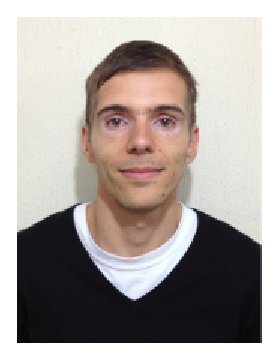
\includegraphics[width=1in,height=1.25in,clip]{Photo_Authors/segura.eps}}]{\bf Carlos Segura} (M'13) was born in Santa Cruz de Tenerife, Spain, on August 03, 1983. He received the M.S. degree in computer science from the Universidad de La Laguna, in 2009 and the Ph.D. degree in computer science from the Universidad de La Laguna, in 2012.
%%
%%He has authored and co-authored over 50 technical papers and book chapters, including 15 journal papers. His publications currently report over 300 citations in {\em Google Scholar} and his h-index is 12. Currently he serves in the editorial board of several international conferences. His main research interests are: design of evolutionary algorithms, diversity management and problem solving paradigms.
%%
%%Dr. Segura is a {\em Member} of the IEEE and a member of the ACM. He is currently an Associate Researcher of the Computer Science area at the Centre for Research in Mathematics.
%%
%%\end{IEEEbiography}
%%
%%\begin{IEEEbiography}[{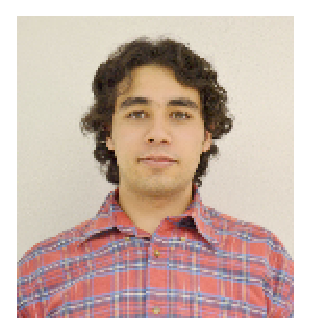
\includegraphics[width=1in,height=1.25in,clip]{Photo_Authors/joel.eps}}]{Joel Chac\'on}
%%recieved the master's degree in computer science from the Center for Research in Mathematics, M\'exico, in 2017, where he is currently working toward the Ph.D. degree.
%%%
%%His main research areas are evolutionary computation, multi-objective optimization, and metaheuristics.
%%\end{IEEEbiography}
%%
%%% if you will not have a photo at all:
%%\begin{IEEEbiography}[{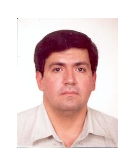
\includegraphics[width=1in,height=1.25in,clip]{Photo_Authors/coello.eps}}]{\bf Carlos A. Coello Coello} received PhD
%%degree in computer science from Tulane University, USA, in 1996.
%%He is currently Professor (CINVESTAV-3F Researcher)
%%and Chair of the Computer Science Department of CINVESTAV-IPN,
%%in Mexico City, M\'{e}xico.
%%
%%Dr. Coello has authored and co-authored over 450
%%technical papers and book chapters. He has also co-authored the
%%book {\em Evolutionary Algorithms
%%for Solving Multi-Objective Problems} (Second Edition,
%%Springer, 2007).
%%His publications currently report over 29,000 citations
%%in {\em Google Scholar} (his h-index is 67).
%%Currently, he is associate editor of the 
%%{\em IEEE Transactions on Evolutionary Computation}
%%and serves in the editorial board of 12 other
%%international journals. 
%%His major research interests are: evolutionary multi-objective
%%optimization and constraint-handling techniques for evolutionary algorithms.
%%
%%He received the {\em 2007 National
%%Research Award} from the Mexican Academy of Sciences
%%in the area of {\em Exact Sciences} and the 
%%{\em Medal to the Scientific Merit 2009}, granted by Mexico
%%City's congress. He is a {\em Fellow} of the IEEE, and a member of
%%the ACM, Sigma Xi, and the Mexican Academy of Science.
%%\end{IEEEbiography}

%\begin{IEEEbiography}[{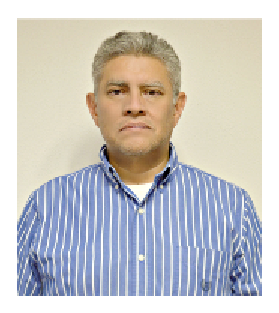
\includegraphics[width=1in,height=1.25in,clip]{Photo_Authors/hernandez.eps}}]{\bf Arturo Hern\'andez Aguirre} received the PhD degree in Computer Science from Tulane University in 2001.
%
%He is the author of over 30 journal papers and over 100 conference papers. He has edited 2 books of the Springer series Lecture Notes in Computer Science. He currently serves as associate editor of Computational Optimization and Computation Journal. His main research interests are: i) evolutionary computation algorithms for global and constrained optimization, and ii) estimation of distribution algorithms for global optimization in real parameter space.
%\end{IEEEbiography}

% if you will not have a photo at all:
%\begin{IEEEbiographynophoto}{John Doe}
%Biography text here.
%\end{IEEEbiographynophoto}

% insert where needed to balance the two columns on the last page with
% biographies
%\newpage

%\begin{IEEEbiographynophoto}{Jane Doe}
%Biography text here.
%\end{IEEEbiographynophoto}

% You can push biographies down or up by placing
% a \vfill before or after them. The appropriate
% use of \vfill depends on what kind of text is
% on the last page and whether or not the columns
% are being equalized.

%\vfill

% Can be used to pull up biographies so that the bottom of the last one
% is flush with the other column.
%\enlargethispage{-5in}



% that's all folks
\end{document}


